\chapter{Dataset and preprocessing}\label{chapter4}
\section{Dataset}
We have chosen the EyePACS dataset \cite{cuadros2009eyepacs} to train our model. This dataset was offered for the \textit{Diabetic retinopathy detection} Kaggle competition \cite{diabeticretinopathydetection}  and can be freely used for research after accepting the conditions of the competition.

\begin{figure}[tbp]
    \centering
    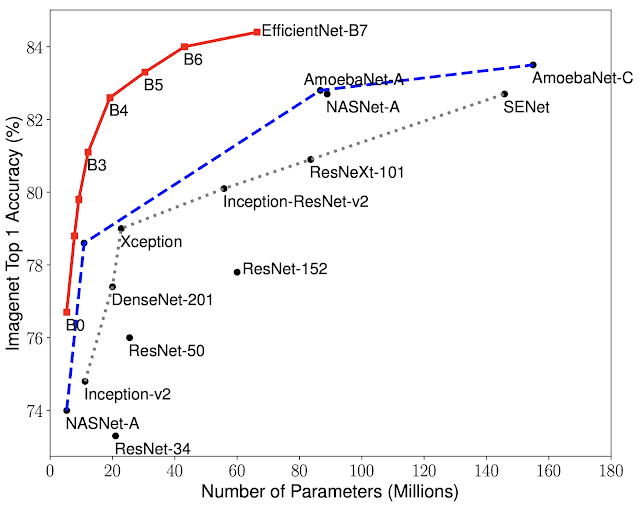
\includegraphics[width=\textwidth]{figures/chapter4/Dataset/comparison.jpg}
    \caption{Inverted and non-inverted image. Optic disk (green) and torch (red) are highlighted.}
    \label{fig:inverted}
\end{figure}

The dataset has a total of 88.704 fundus images, divided into two sets: a training set consisting of 35.126 images and a test with 53.578 files, summing a total of 88 GB. The images include the left and right eye for each of the 44.352 observed patients. 

The images come from a variety of cameras and may have different colors, resolutions, and capture different part of the eyes. Some images also contain significant noise, in the shape of under or overexposure, reflections or other graphical artifacts.

Different images may also have different orientations, depending on the type of equipment used to take the photograph. Some images are anatomically oriented (for the right eye, the macula is on the left and the optic nerve is on the right or there is a notch on the side of the image) and others are mirrored, as depicted in \Cref{fig:inverted}.

The resolution of images is quite varied: for the training set, the width of the images is between 400 and 5184 pixels with a mean of 3637 pixels and the height between 289 and 3.456 with a mean of 2.473 pixels. The relationship between width and height (the aspect ratio) is also remarkably different between images, which means the images cannot be directly resized to a common size without heavily distorting some of them.

All the images are compressed as JPEG and the image size is between 0.01 and 2.07 Megabytes with a mean of 1.03 Megabytes.

\begin{figure}[htbp]
     \begin{subfigure}[b]{0.19\textwidth}
         \centering
         \includegraphics[width=\textwidth, height=\textwidth]{figures/chapter4/Dataset/noDR/41_left.jpeg}
    \end{subfigure}
    \hfill
    \begin{subfigure}[b]{0.19\textwidth}
         \centering
         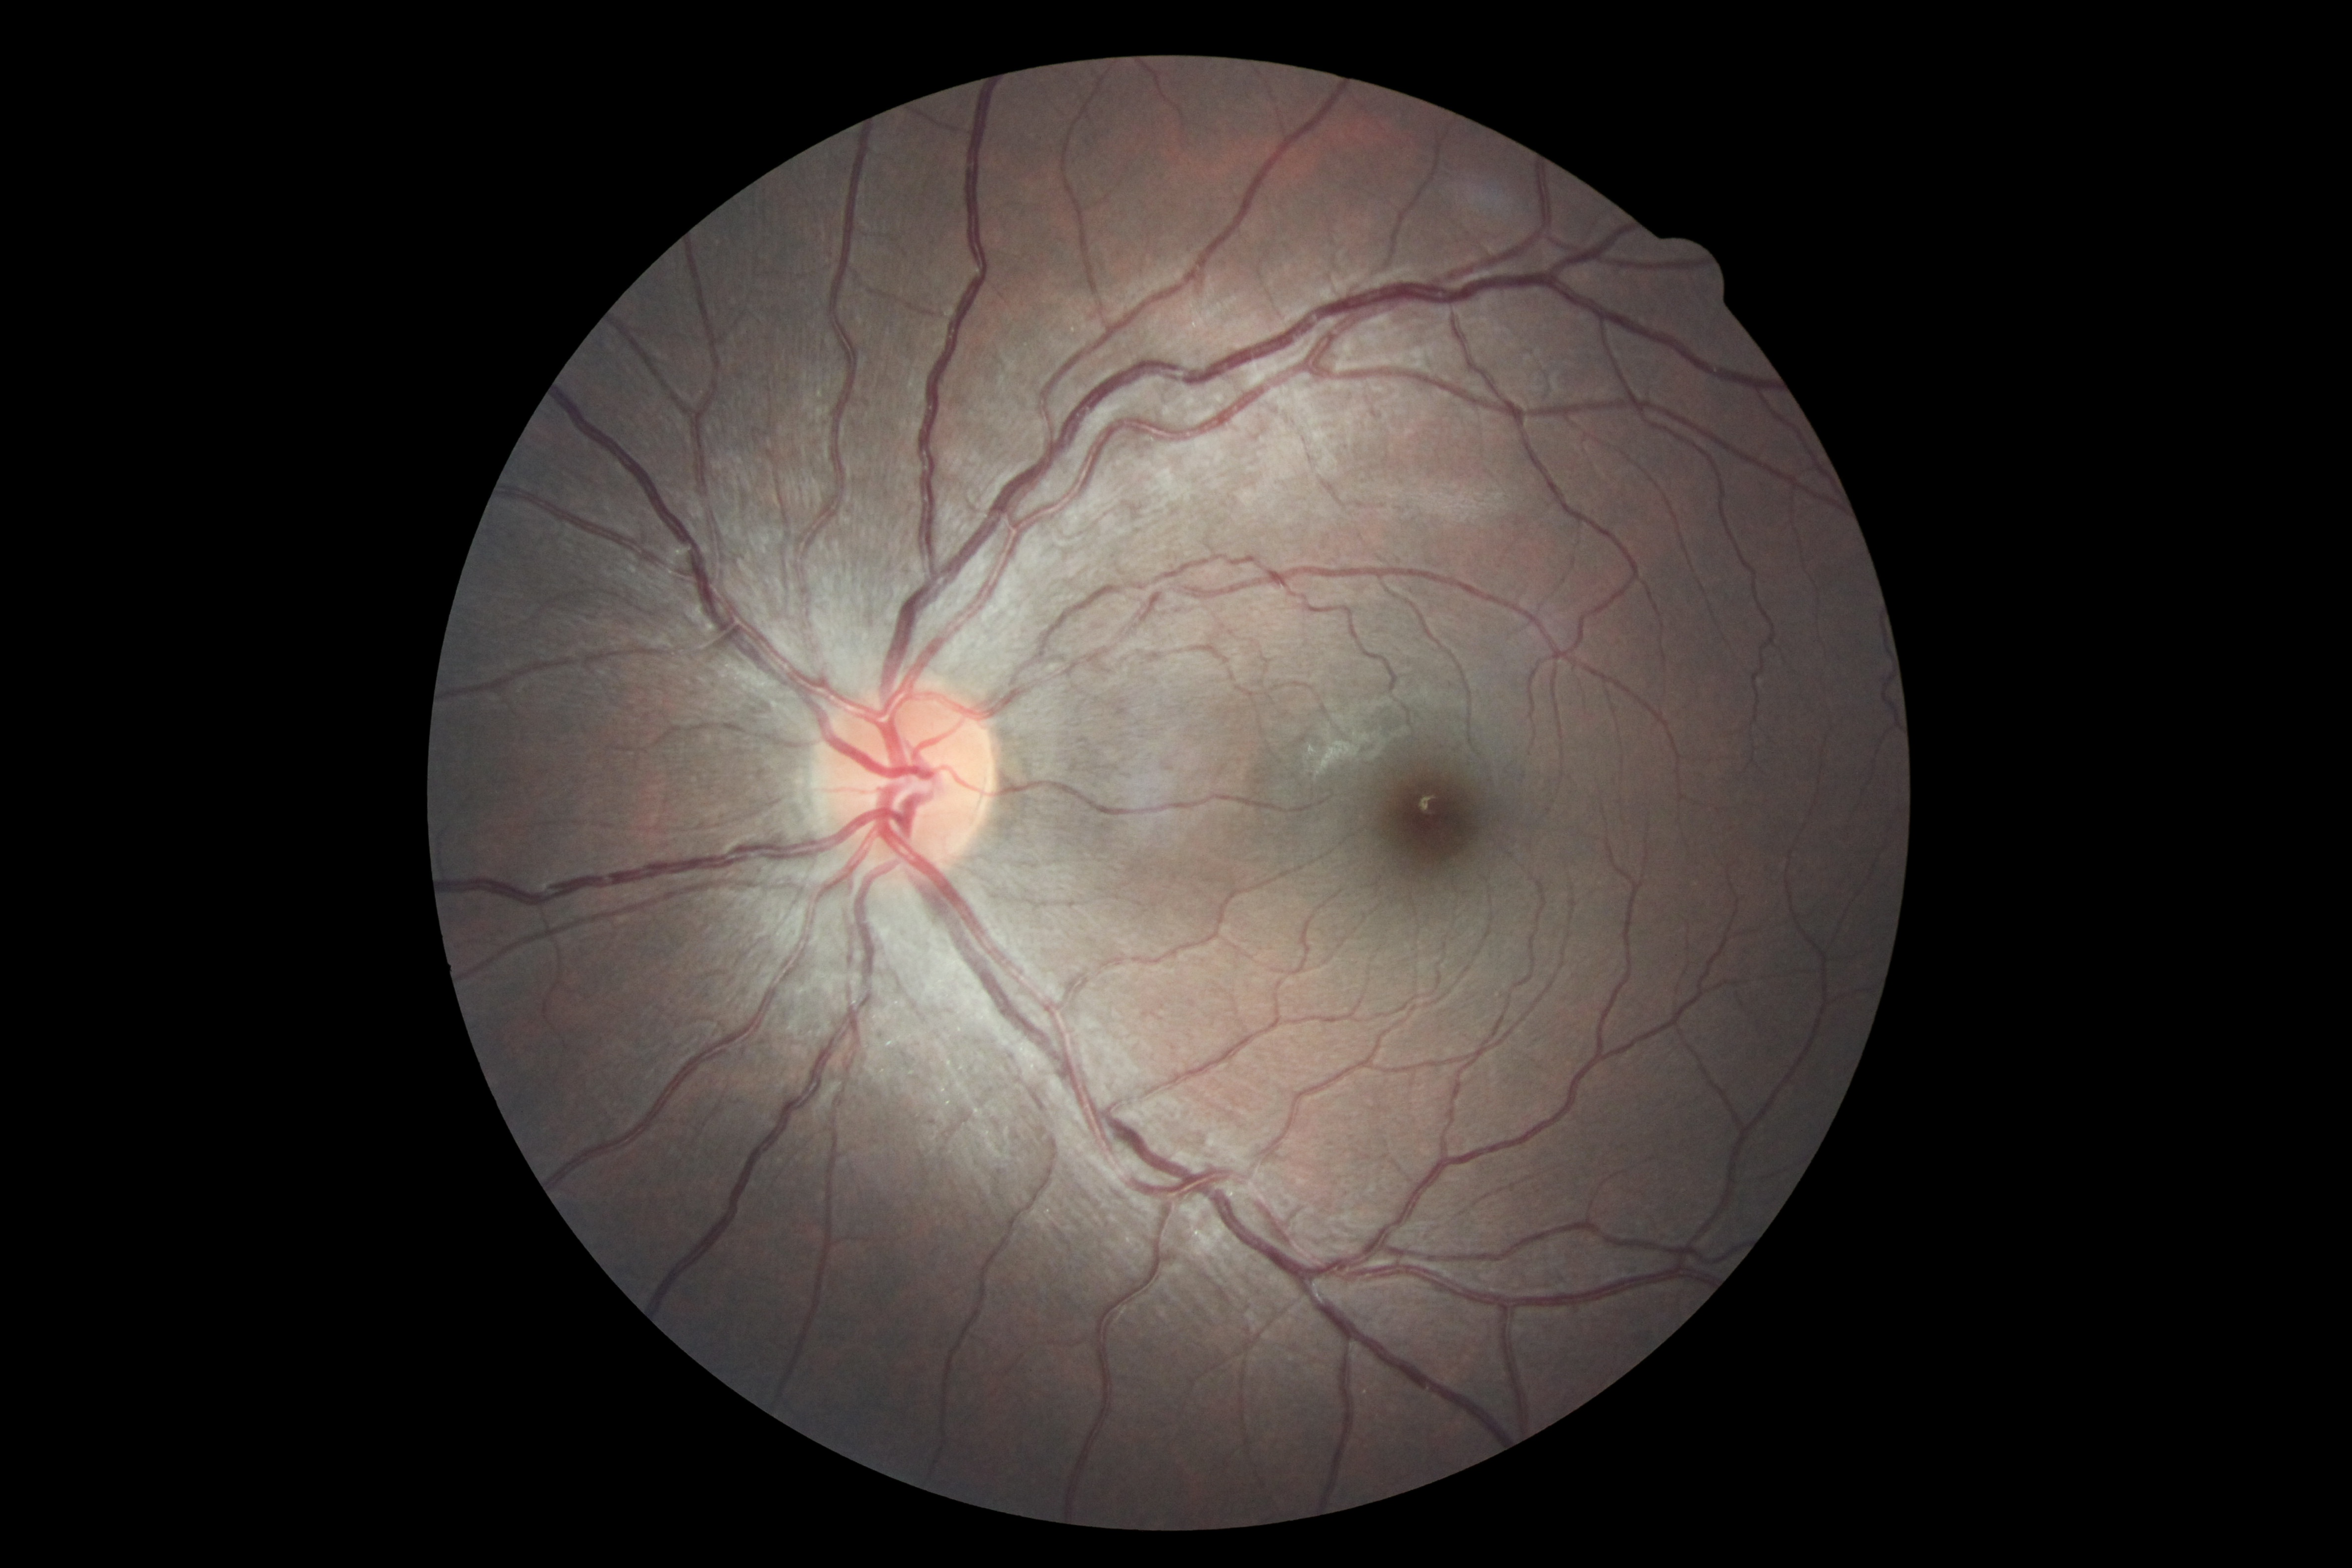
\includegraphics[width=\textwidth, height=\textwidth]{figures/chapter4/Dataset/mild/114_left.jpeg}
    \end{subfigure}
    \hfill
    \begin{subfigure}[b]{0.19\textwidth}
         \centering
         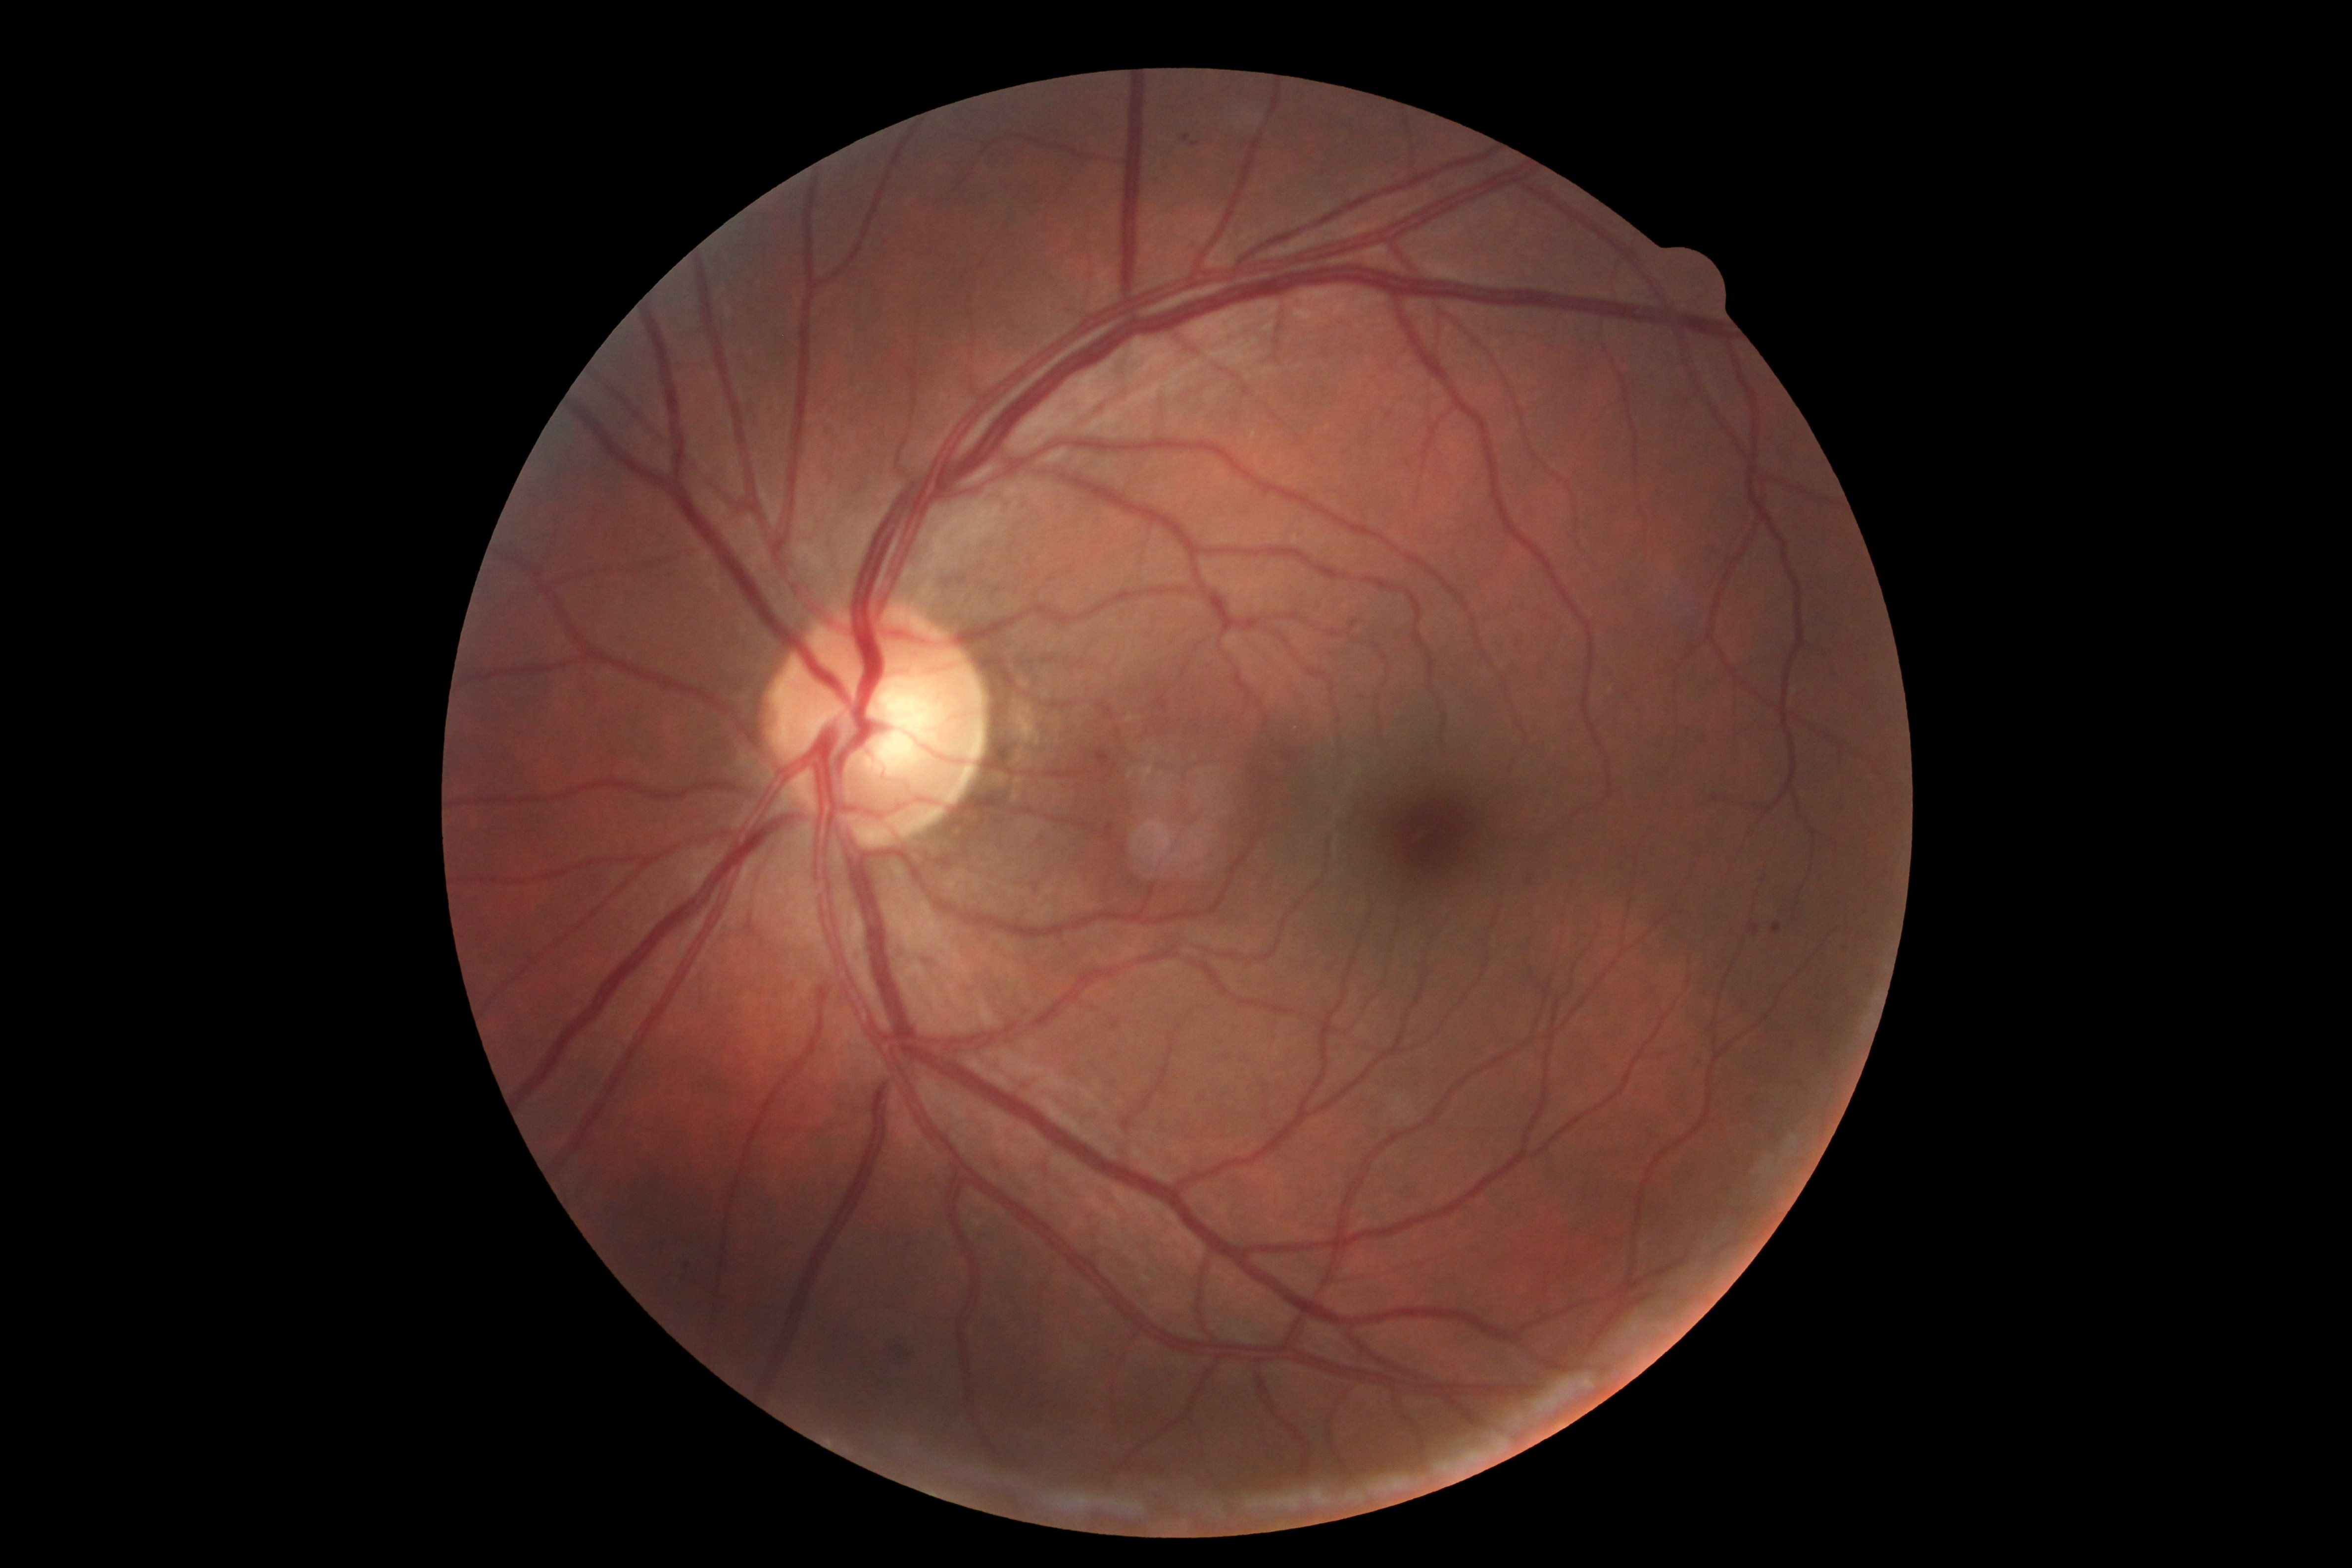
\includegraphics[width=\textwidth, height=\textwidth]{figures/chapter4/Dataset/moderate/129_left.jpeg}
    \end{subfigure}
    \hfill
    \begin{subfigure}[b]{0.19\textwidth}
         \centering
         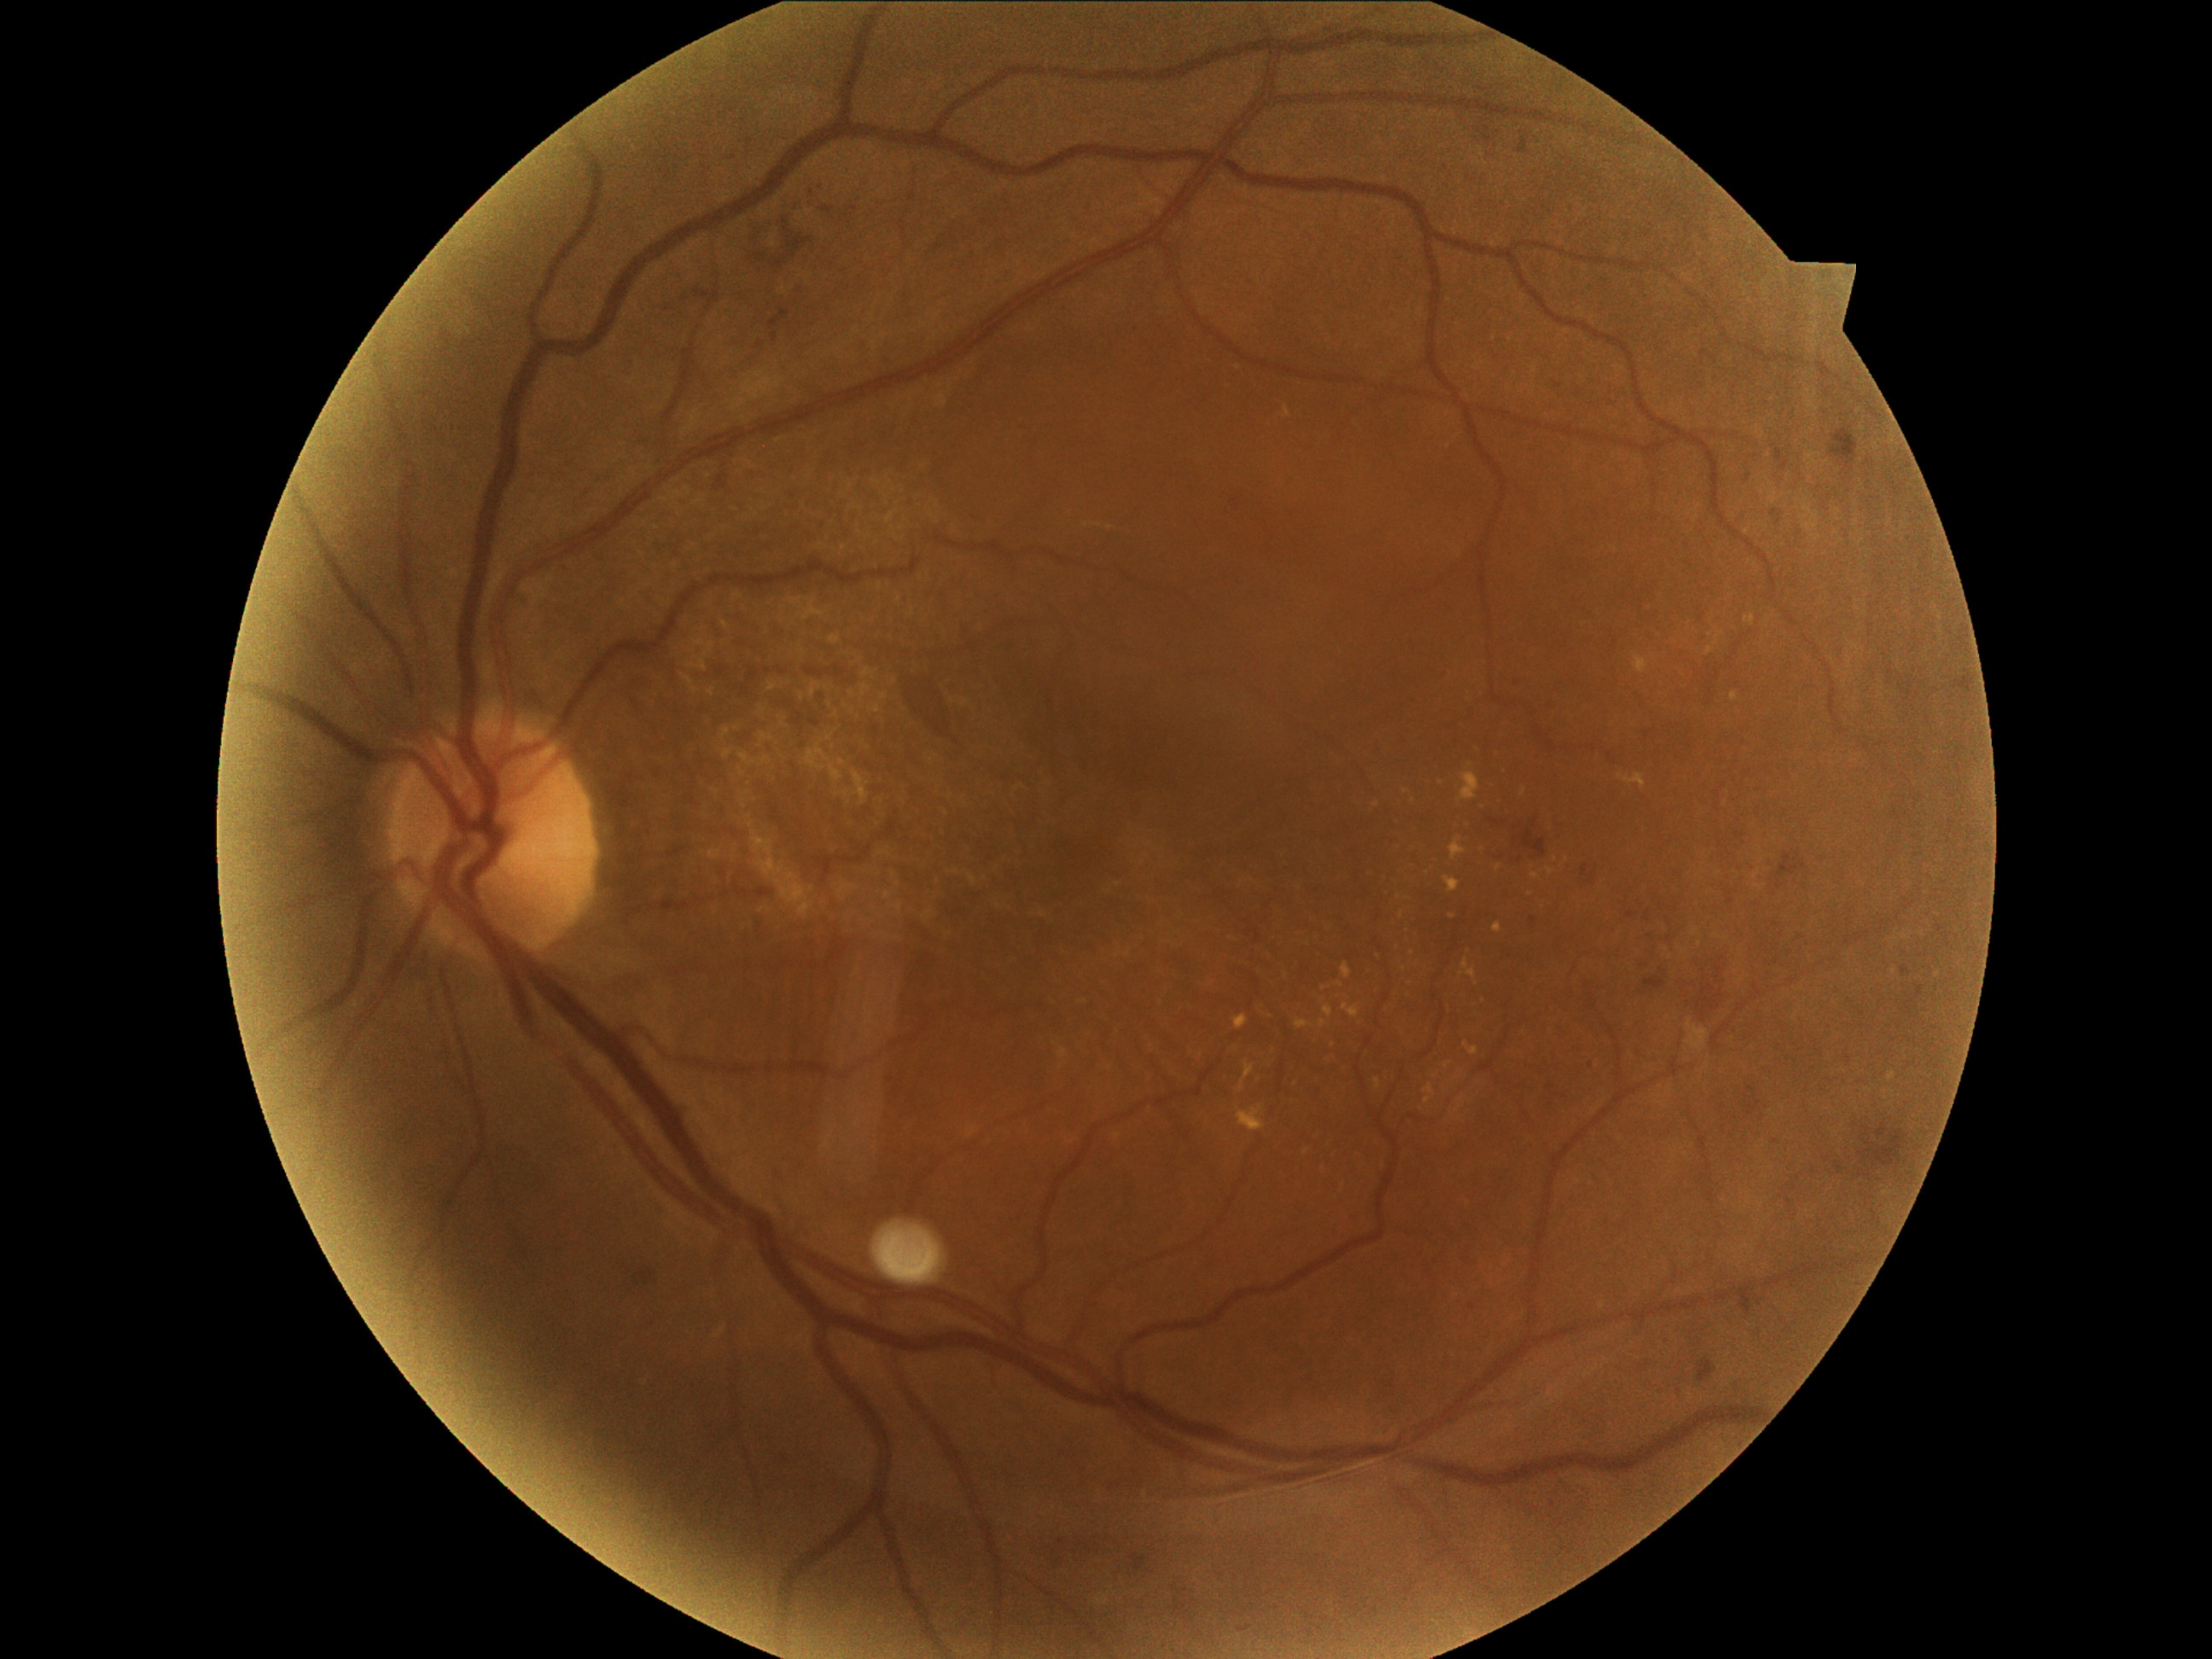
\includegraphics[width=\textwidth, height=\textwidth]{figures/chapter4/Dataset/severe/163_left.jpeg}
     \end{subfigure}
     \hfill
     \begin{subfigure}[b]{0.19\textwidth}
         \centering
         \includegraphics[width=\textwidth, height=\textwidth]{figures/chapter4/Dataset/proliferative/294_left.jpeg}
     \end{subfigure}

    \bigskip
     \begin{subfigure}[b]{0.19\textwidth}
         \centering
         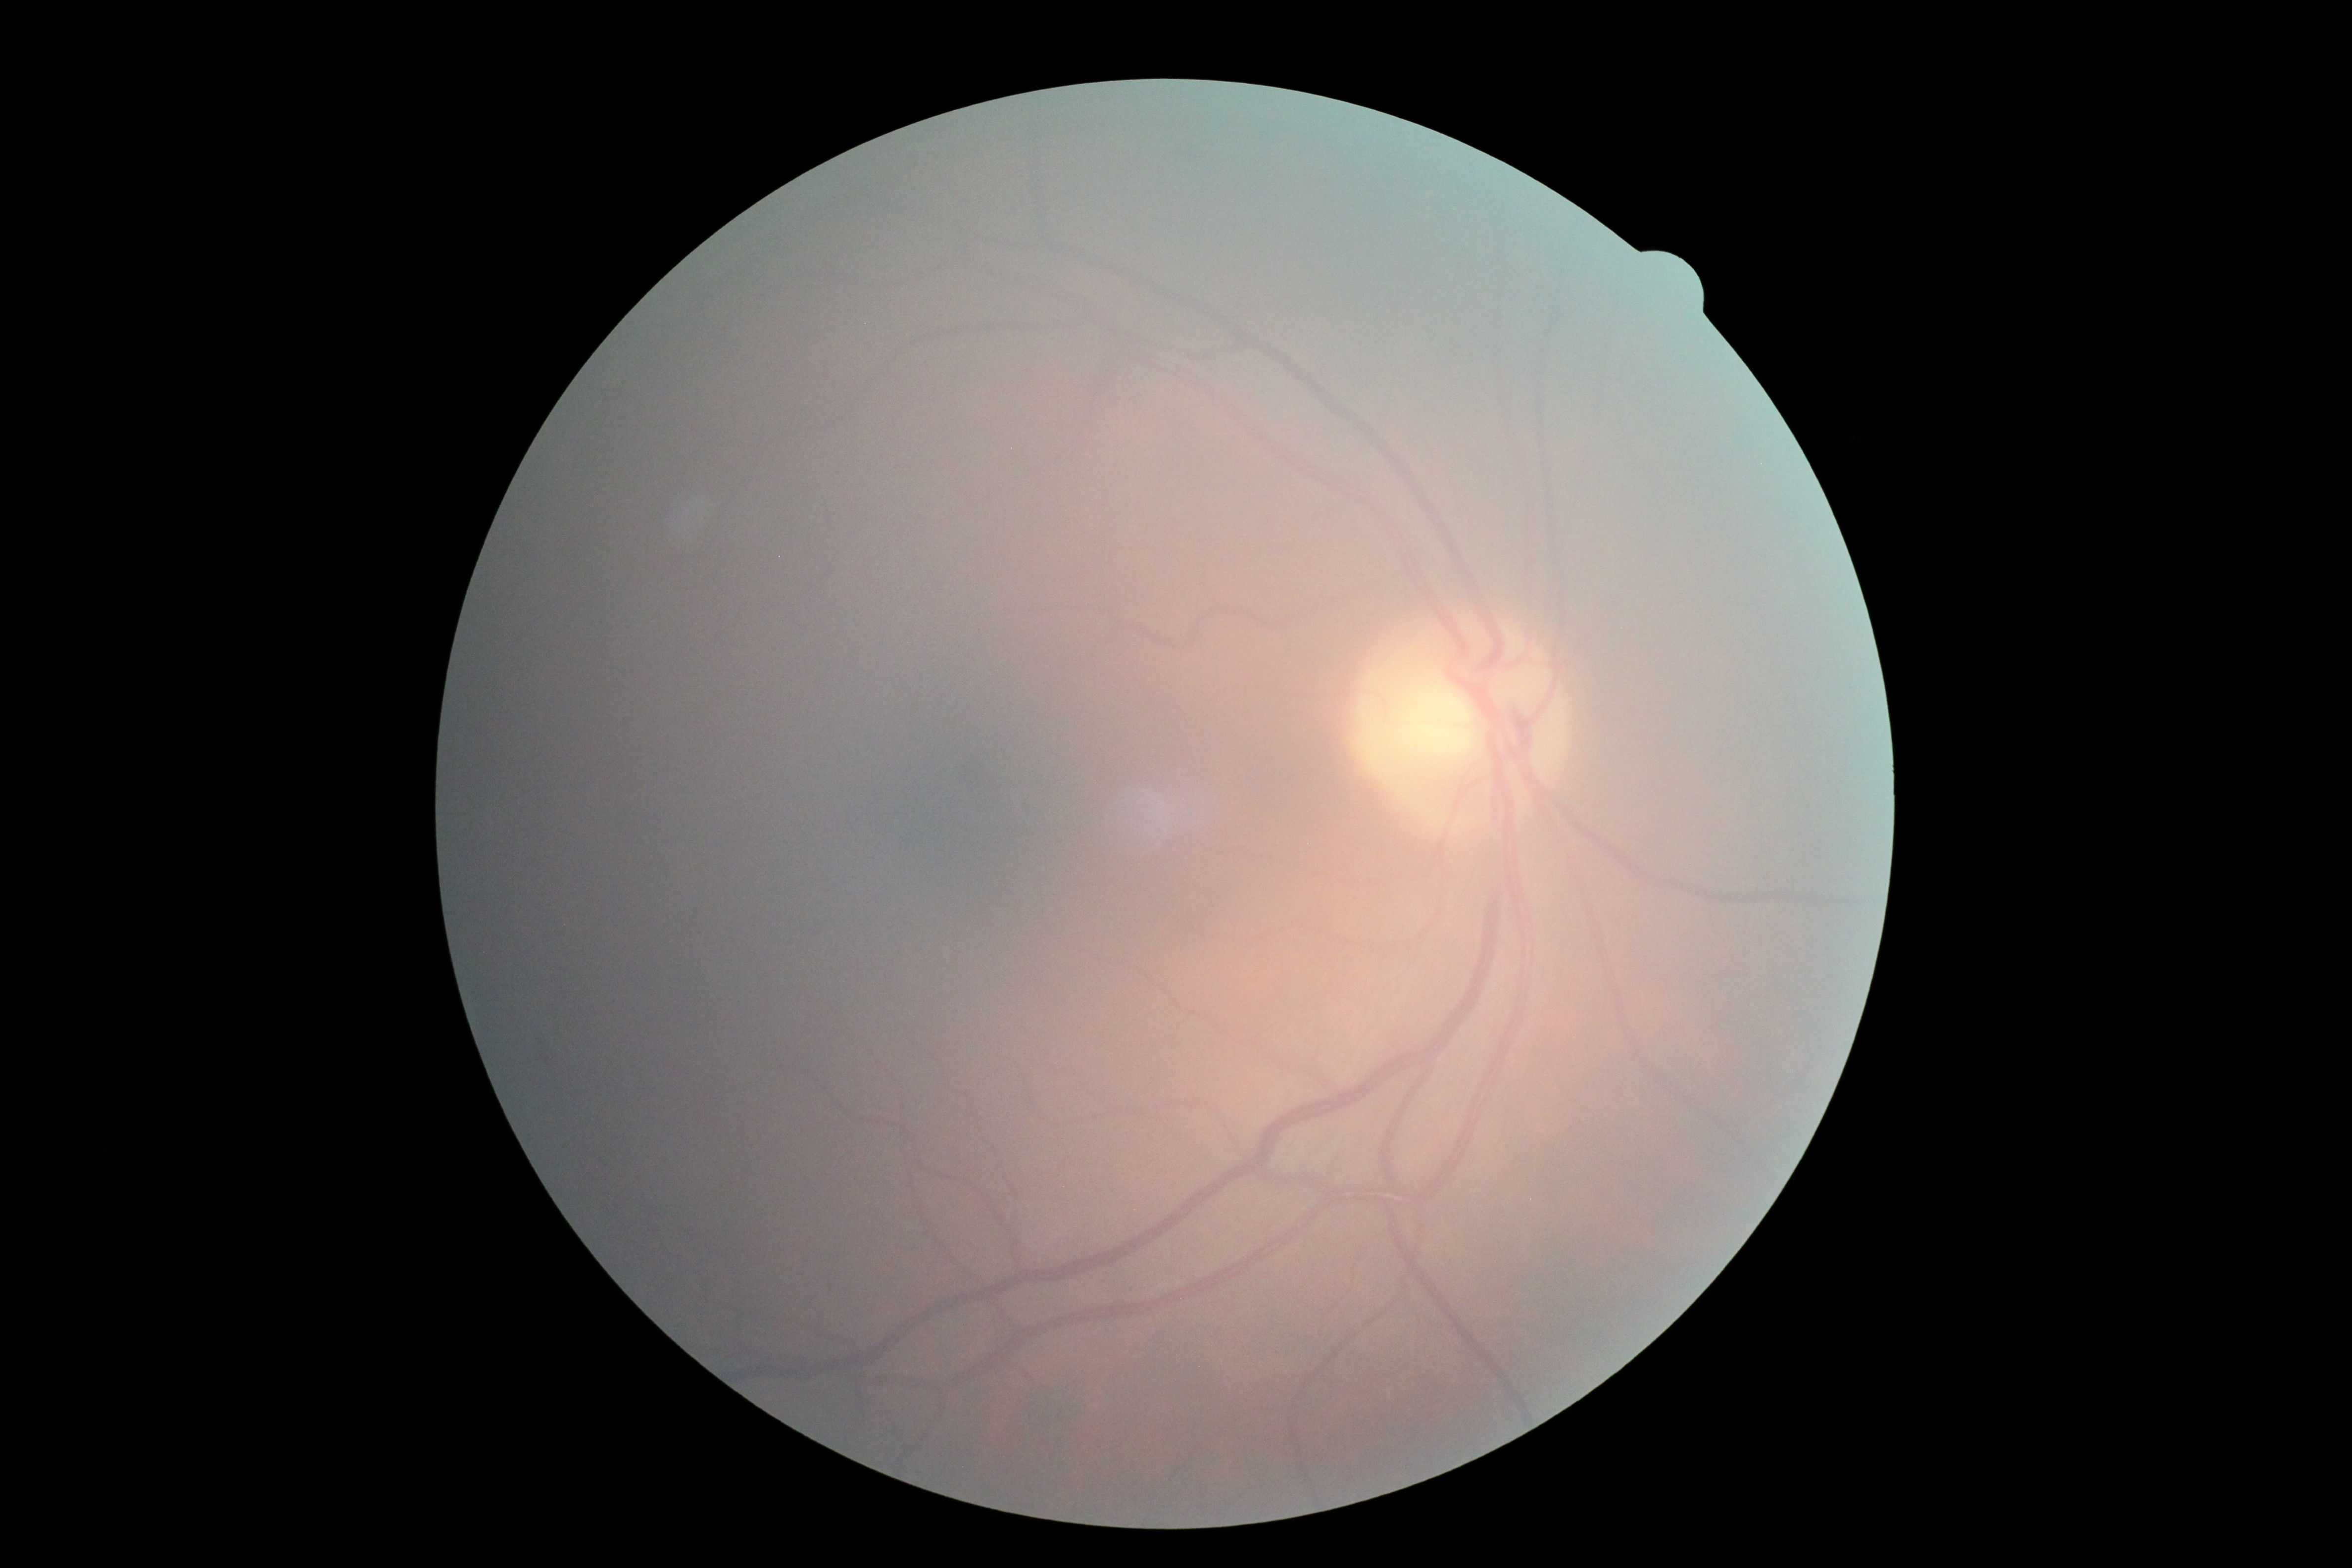
\includegraphics[width=\textwidth, height=\textwidth]{figures/chapter4/Dataset/noDR/75_right.jpeg}
         \caption{Grade 0}
    \end{subfigure}
    \hfill
    \begin{subfigure}[b]{0.19\textwidth}
        \centering
        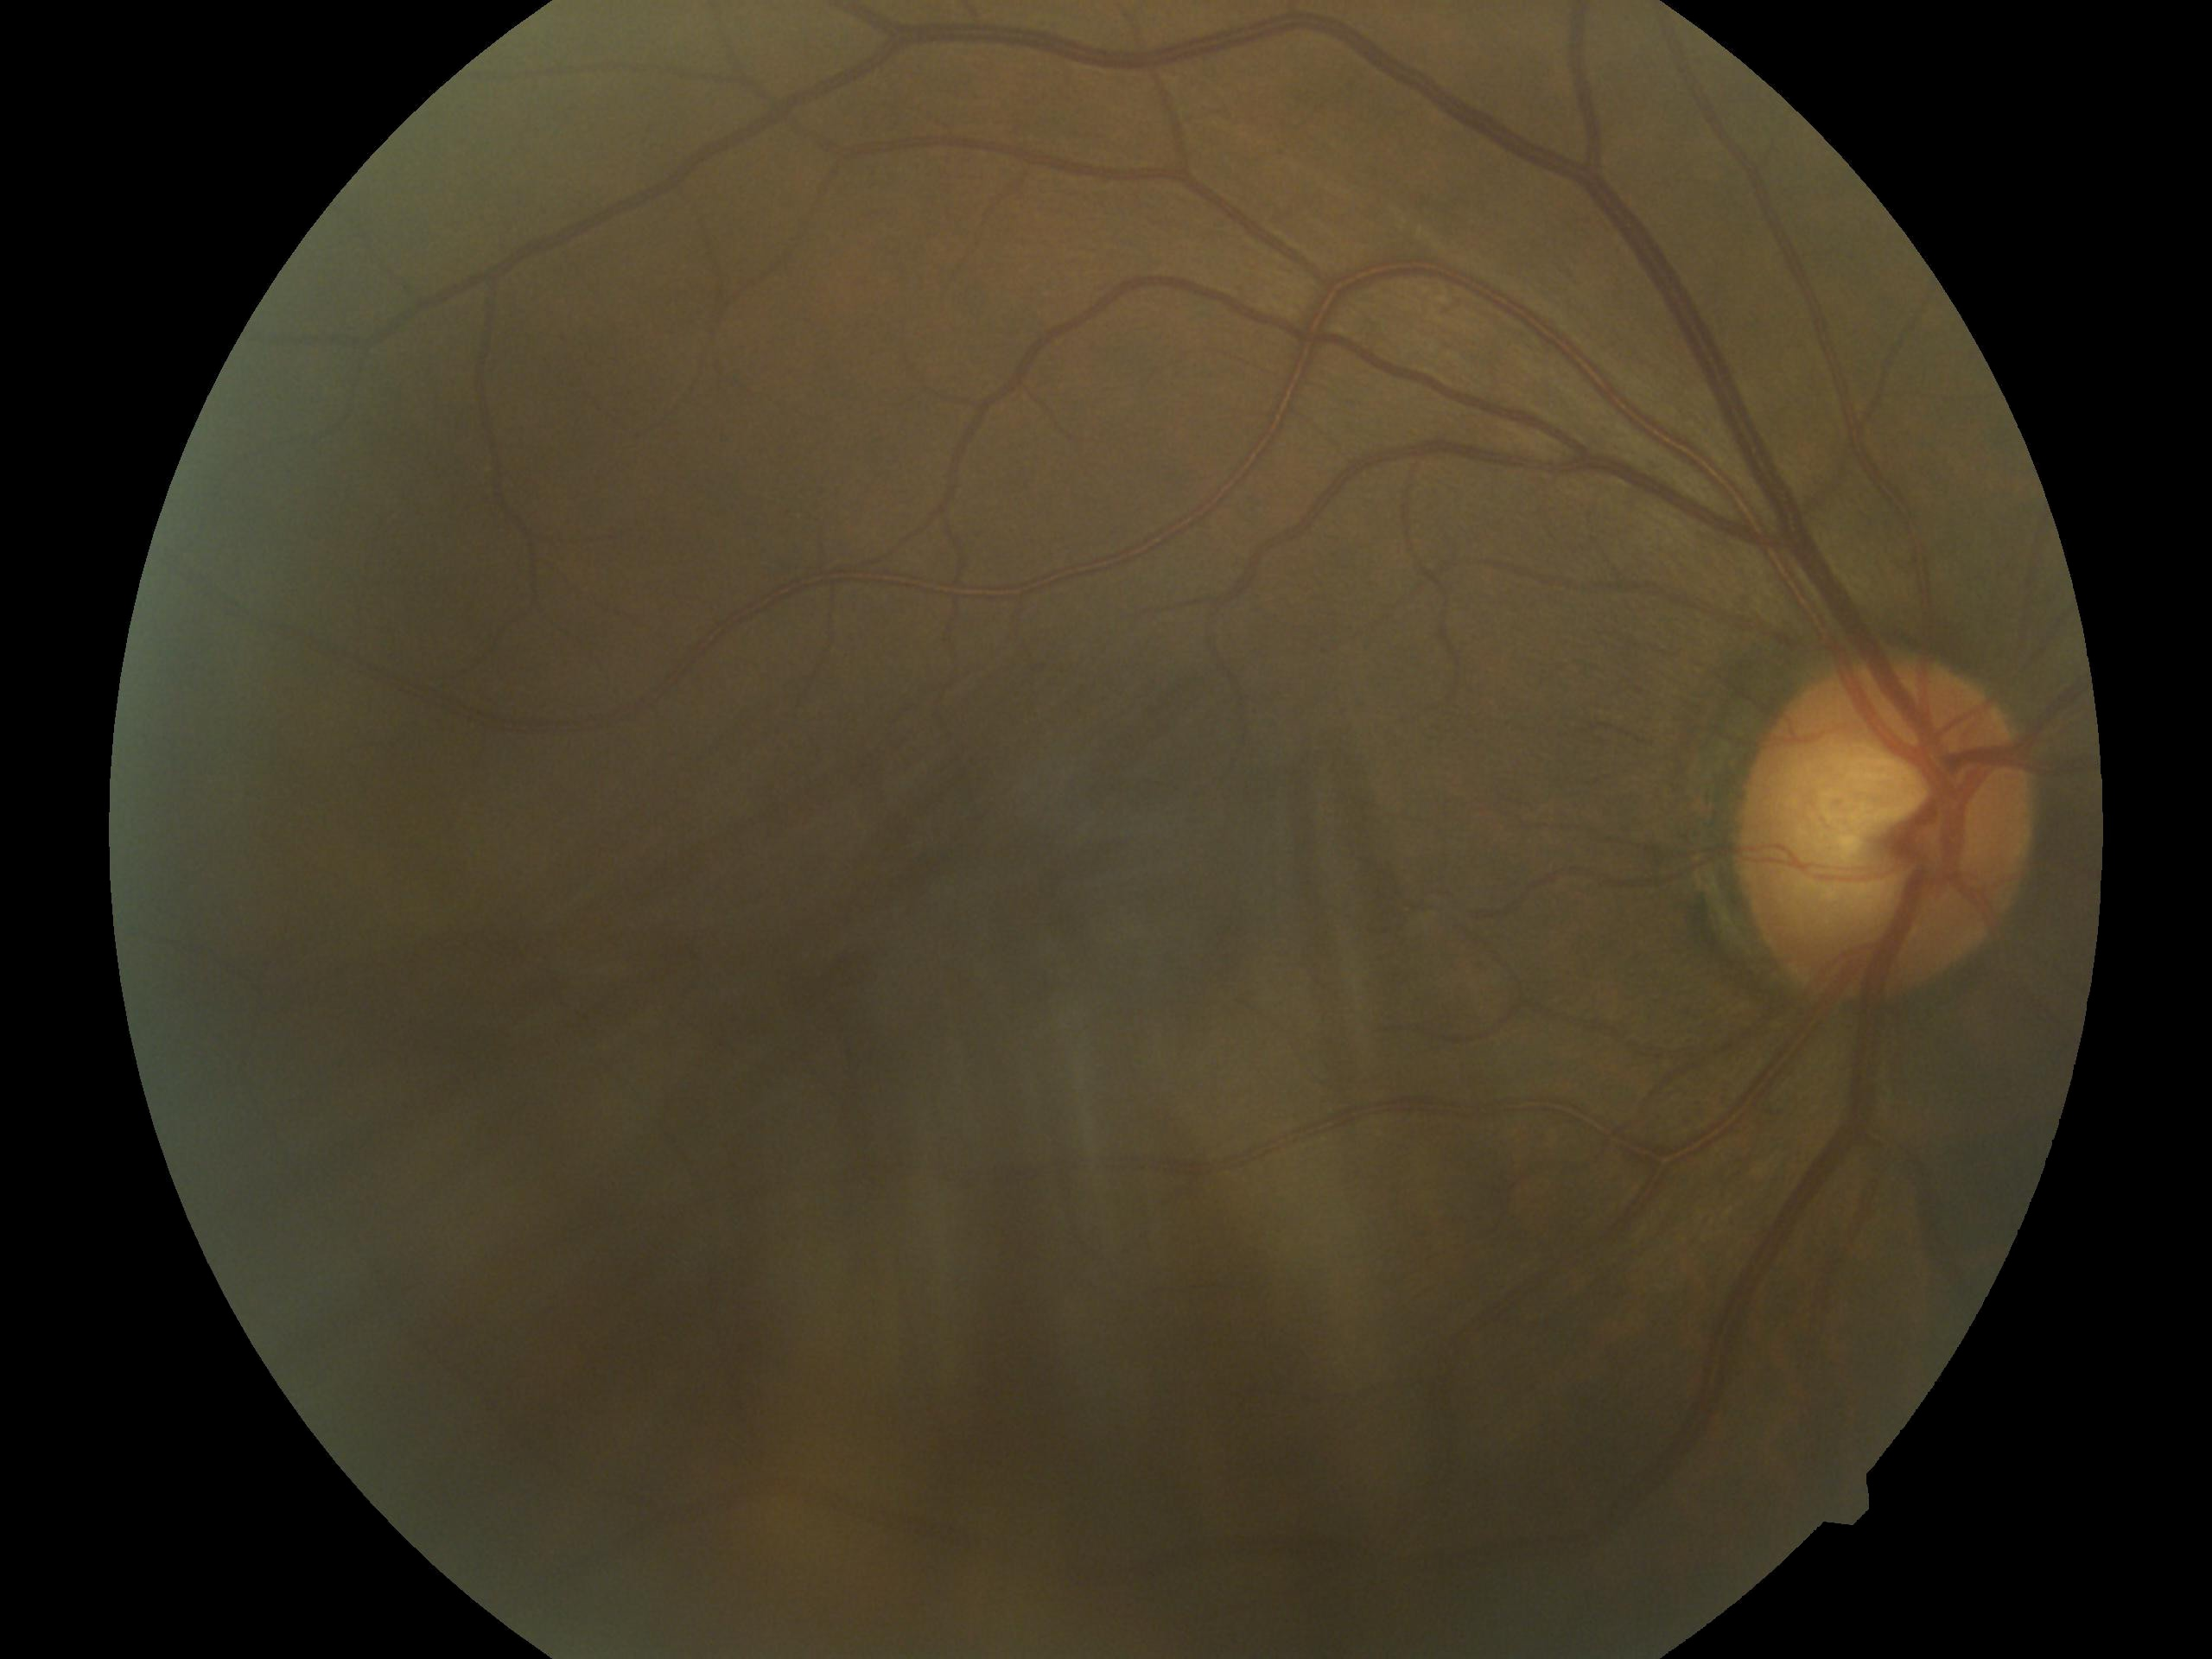
\includegraphics[width=\textwidth, height=\textwidth]{figures/chapter4/Dataset/mild/36_right.jpeg}
        \caption{Grade 1}
    \end{subfigure}
    \hfill
    \begin{subfigure}[b]{0.19\textwidth}
        \centering
        \includegraphics[width=\textwidth, height=\textwidth]{figures/chapter4/Dataset/moderate/54_right.jpeg}
        \caption{Grade 2}
    \end{subfigure}
    \hfill
    \begin{subfigure}[b]{0.19\textwidth}
        \centering
        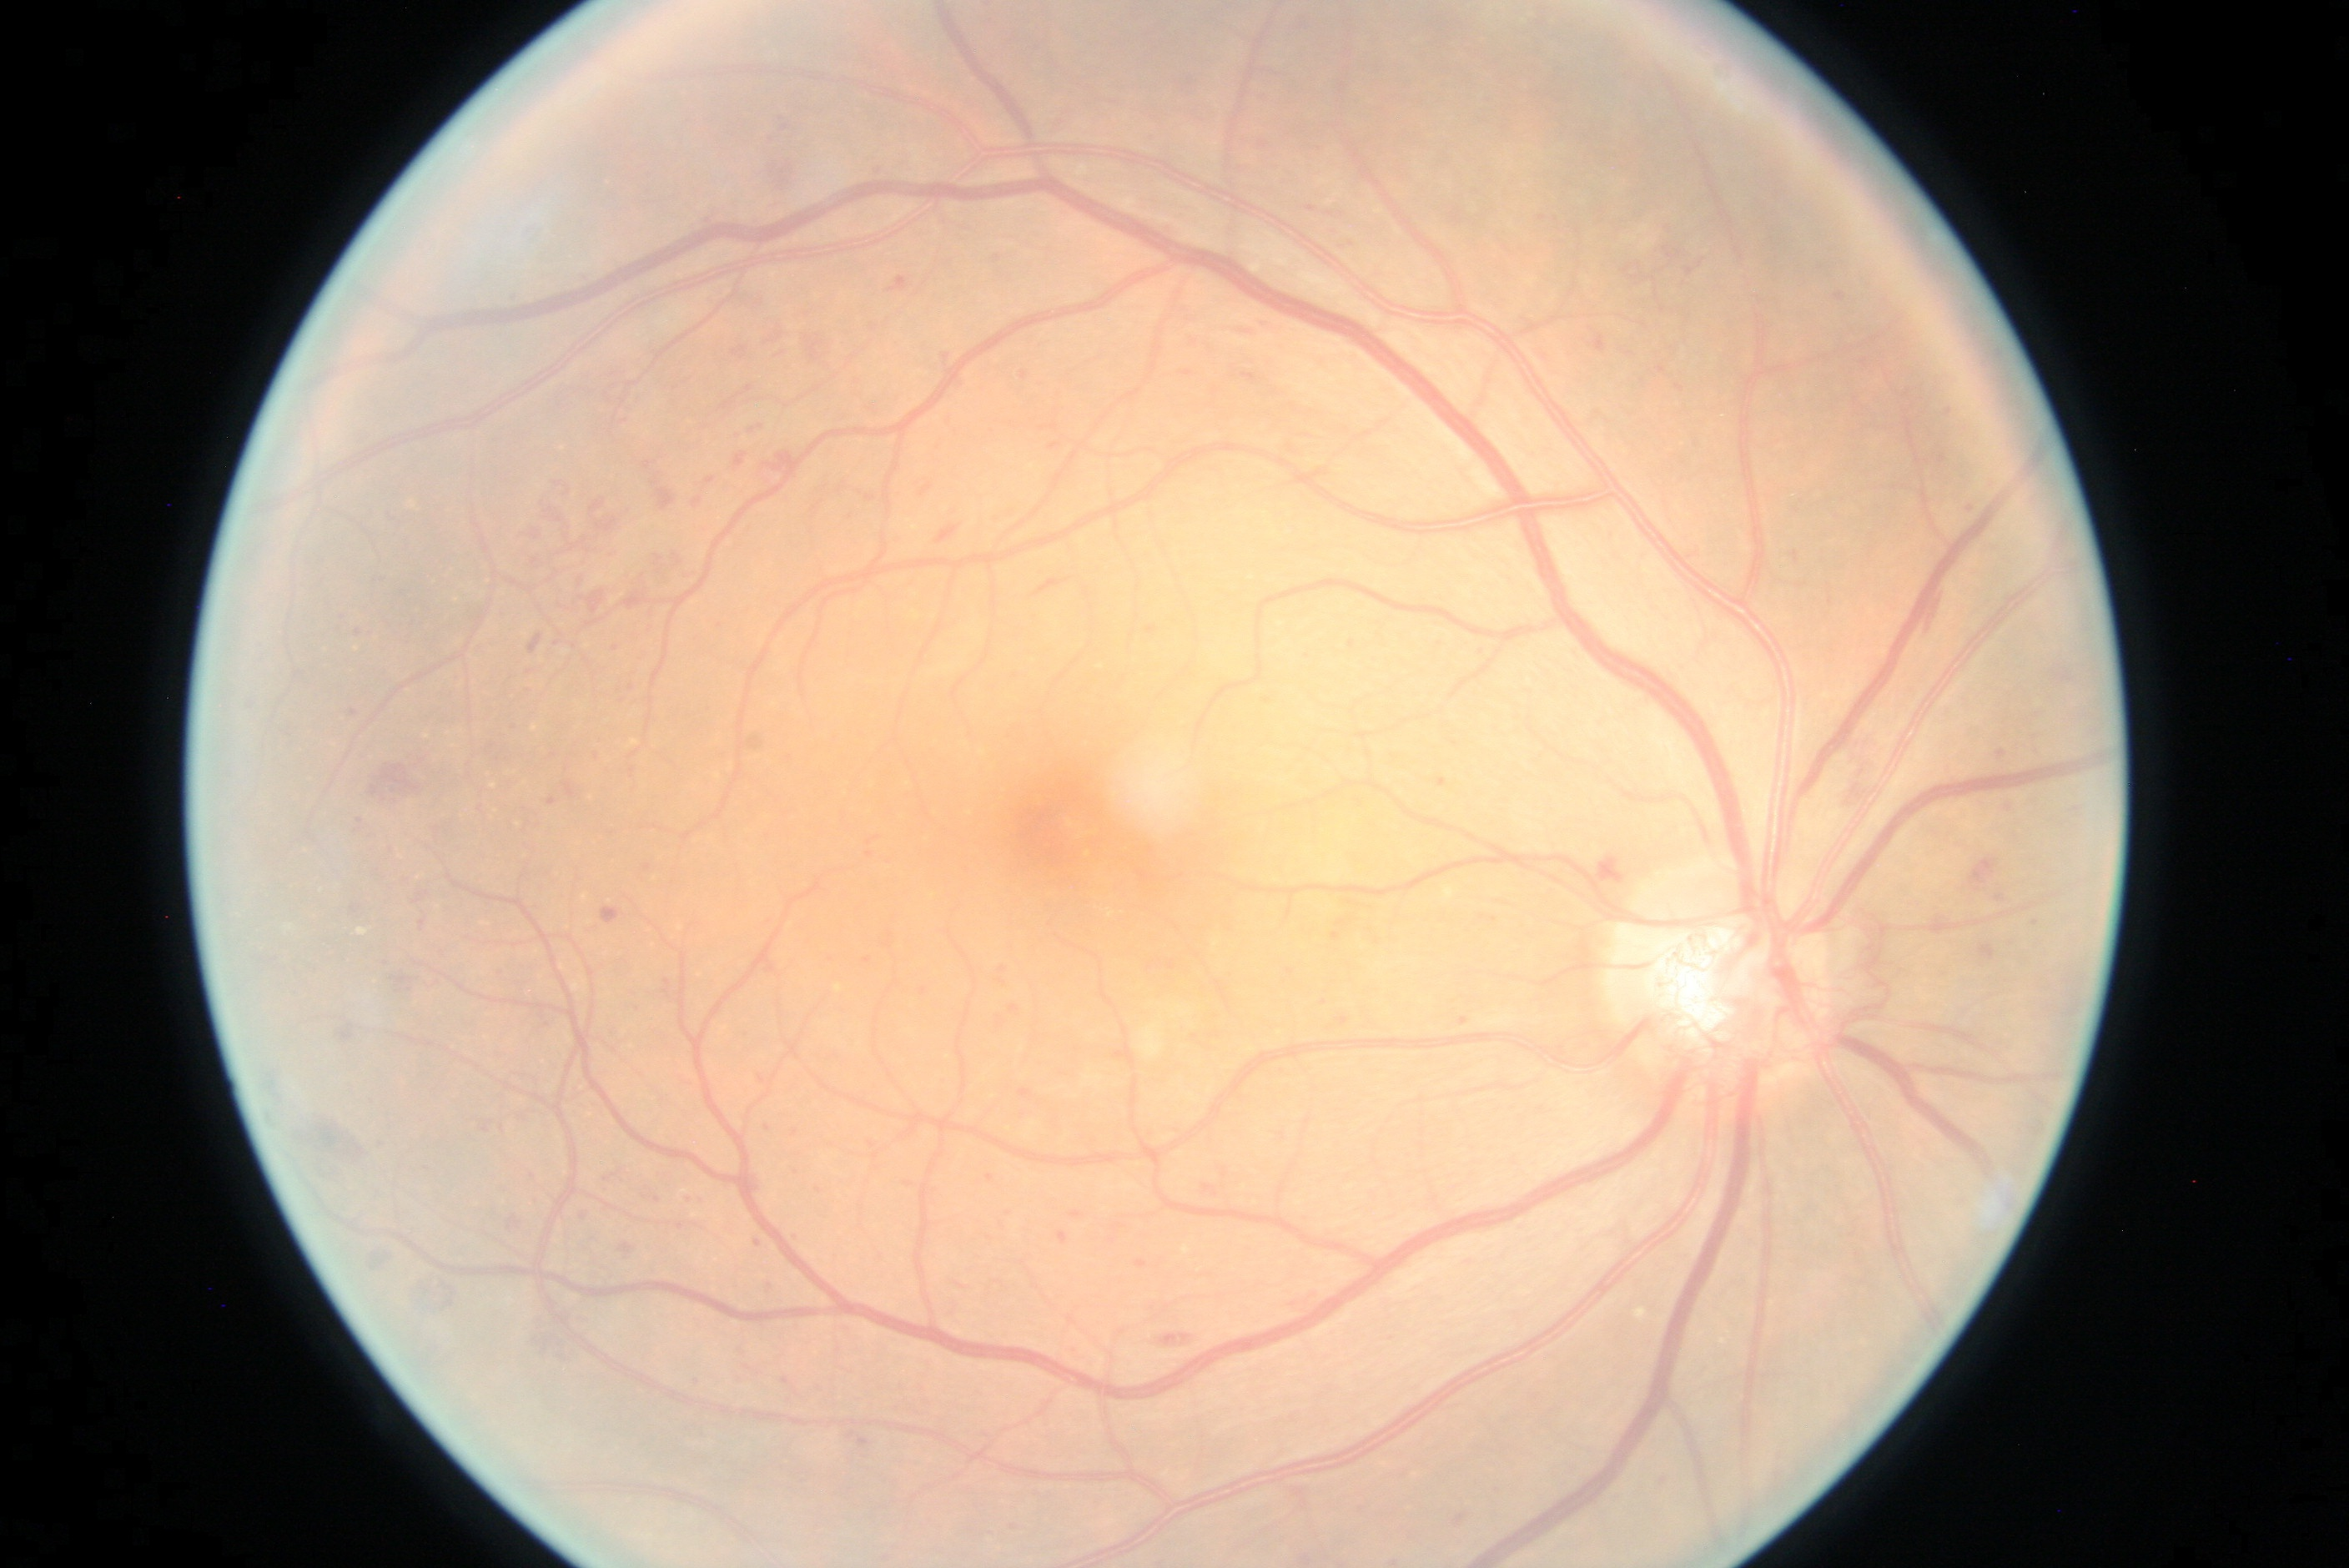
\includegraphics[width=\textwidth, height=\textwidth]{figures/chapter4/Dataset/severe/326_right.jpeg}
        \caption{Grade 3}
     \end{subfigure}
     \hfill
     \begin{subfigure}[b]{0.19\textwidth}
        \centering
        \includegraphics[width=\textwidth, height=\textwidth]{figures/chapter4/Dataset/proliferative/352_right.jpeg}
        \caption{Grade 4}
    \end{subfigure}
    \caption{Example of images of different classes. Note the different color, brightness, and scale of each image. }
    \label{fig:disease_level}
\end{figure}

Both train and test images have been graded for DR by a professional ophthalmologist: the rating is a number between 0 and 4 representing no DR, mild, moderate or severe DR or proliferative DR. The  \Cref{fig:disease_level} shows some examples of images in each of these classes.

\begin{table}[tb]
\centering
\begin{tabular}{|c|c|c|}
\hline
Disease Stage                                                        & Number of Images & Proportion \\ \hline
\hline
\begin{tabular}[c]{@{}c@{}}No apparent \\ retinopathy\end{tabular}   & 25.810            & 73.48\%    \\ \hline
Mild retinopathy                                                     & 5.292             & 15.06\%    \\ \hline
\begin{tabular}[c]{@{}c@{}}Moderate \\ retinopathy\end{tabular}      & 2.443             & 6.95\%     \\ \hline
\begin{tabular}[c]{@{}c@{}}Severe \\ retinopathy\end{tabular}        & 873              & 2.49\%     \\ \hline
\begin{tabular}[c]{@{}c@{}}Proliferative \\ retinopathy\end{tabular} & 708              & 2.02\%     \\ \hline
\end{tabular}
\label{table:classDistribution}
\caption{Distribution of classes in the
dataset. No DR cases are heavily overrepresented}
\end{table}
Concerning class distribution, the dataset is heavily unbalanced, as no DR images account for 73.48\% of the training set, while the Mild, Moderate, Severe and Proliferative DR have a representation of 15.06\%,  6.95\%, 2.49\% and 2.02\% respectively, as depicted in \Cref{table:classDistribution}.

There is a strong correlation between the left and right eye grading (Pearson correlation coefficient \( \rho = 0.85 \)). We find two possible causes behind this phenomenon: in the first place, persistently high sugar levels in blood should damage both retinas at a similar rate, leading to similar levels of DR. In the second place, physicians usually examine both eyes at once, so it is possible that the prediction made for one eye biases the grading of the second. Whatever the cause, it may be worth exploring \textit{binocular} methods, that consider information coming from both eyes for grading.

\section{Preprocessing}
While most CNN models can work with a wide set of image sizes, using a very high resolution is not computationally feasible, especially in the face of limited computational power. Instead of just resizing them, it is convenient to first crop the background, as it provides no information.

However, detecting the background is not straightforward, as its color may differ between images (although it's dark in all cases). Most naive strategies we tried (as detecting the color of the corners) failed in a subset of cases, for example, when the eye is significantly zoomed.

We finally chose a scheme heavily inspired by the one carried by the winner of the Kaggle competition Ben Graham \cite{competitionRep}, consisting in 3 steps implemented using the open source libraries OpenCV \cite{openCv} and Pillow \cite{pillow}:
\begin{enumerate}
    \item \textbf{Scale down the image, so the radius has a fixed length}: to do this, we first identify the background by drawing a horizontal line through the center of the image and reducing each pixel to the sum of the three RGB components.

    Since the background is close to black, the sum of its pixels will have a very low value. We discard them by selecting the pixels whose components sum more than one tenth of the mean sum.

    The resulting line mostly corresponds to the diameter of the eye. We resize both the x and y-axis by a constant factor, so the radius has 300 pixels. The size of the radius should be adjusted depending on the working resolution of choice.
    
    \item \textbf{Overlap Gaussian noise over the image}: Gaussian noise is created by applying a convolution to the image with a Gaussian kernel, a kernel created by extracting values from a \( \normal(\eta = 0, \sigma = 10) \) distribution, which can be readily done using \( \texttt{gaussianBlur} \) method from OpenCV. 

    We then combine the original and the blurred images using an affine combination, so the final image is equal to \( \alpha I_0 + \beta I_G + \gamma \), where \( I_0 \) is the original image, \( I_G \) the blurred one and \( \alpha = 4, \beta = -4, \gamma = 128\) (the operation is applied independently for each channel). This operation can be done using the \( \texttt{addWeighted} \) method from OpenCV.

    Since \( I_G \) is the blurred version of the original image, the operation is approximately similar to subtracting the local average color. Pixels with a color similar to average one will become gray (color (128, 128, 128)) while pixels with a color different from the surrounding one will remain distinctive. This is especially useful to highlight blood vessels and lesions. 
    
    \item \textbf{Homogenize the background and crop}: we draw a circle in the center of the image, with radius equal to \( 0.9 \) times the radius of the eye (300 pixels). We then set all the pixels outside the circle to a constant color (128, 128, 128).

    To crop the background it is now sufficient to select the smallest bounding box containing all pixels different from the background color, which is straightforward using the \texttt{bbox} method from Pillow.
\end{enumerate}


\begin{figure}[tb]
     \begin{subfigure}[b]{0.24\textwidth}
         \centering
         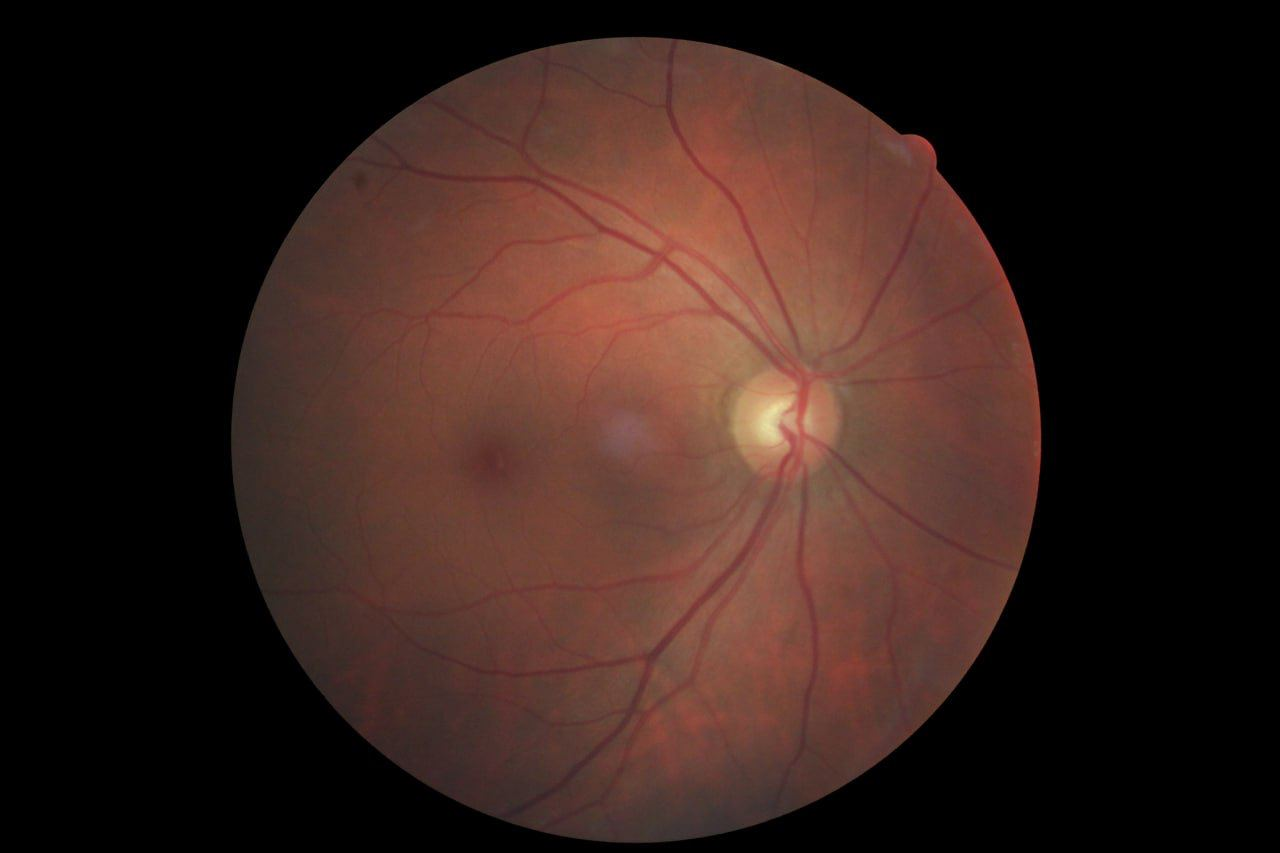
\includegraphics[width=\textwidth, height=\textwidth]{figures/chapter4/Preprocessing/original.jpg}
         \caption{Original}
    \end{subfigure}
     \hfill
         \begin{subfigure}[b]{0.24\textwidth}
        \centering
        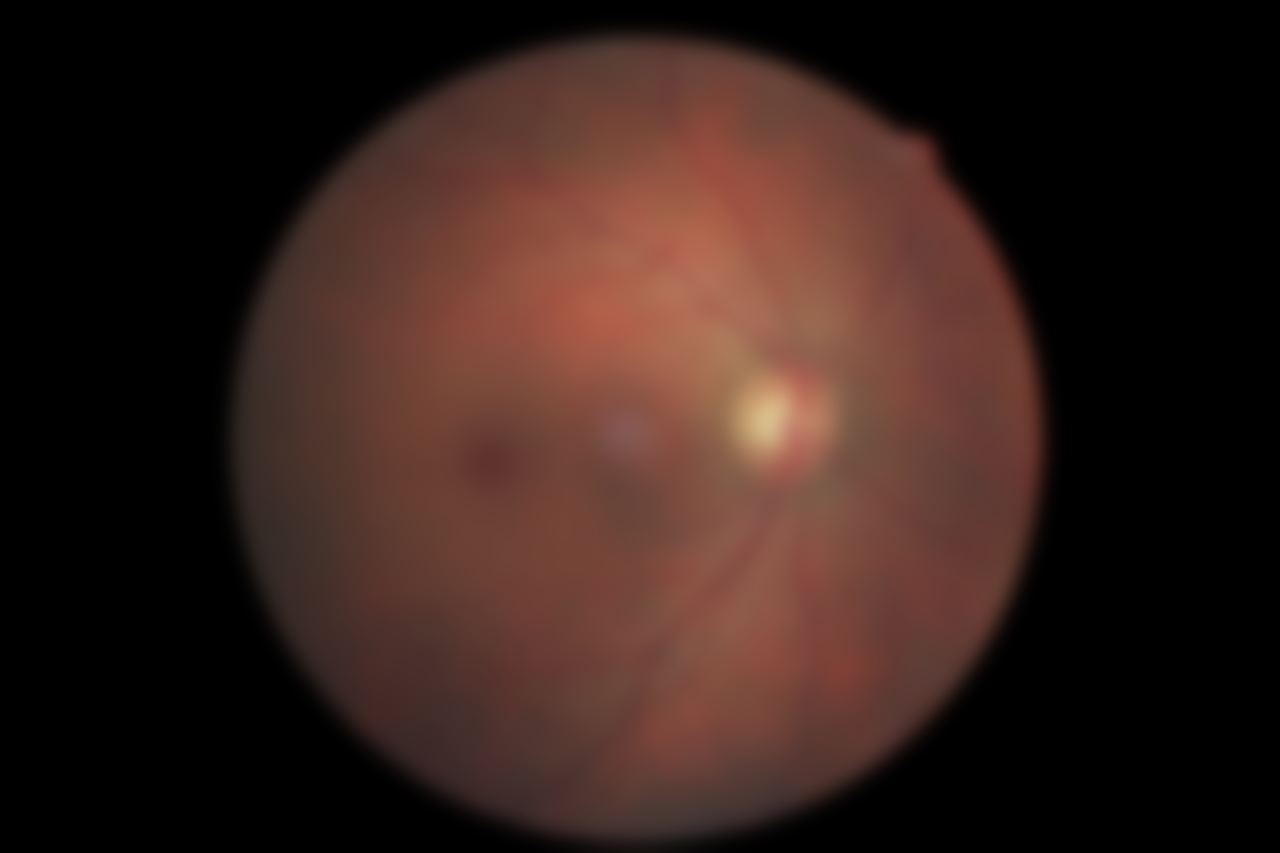
\includegraphics[width=\textwidth, height=\textwidth]{figures/chapter4/Preprocessing/blurred.jpg}
        \caption{Blurred}
    \end{subfigure}
    \hfill
     \begin{subfigure}[b]{0.24\textwidth}
        \centering
        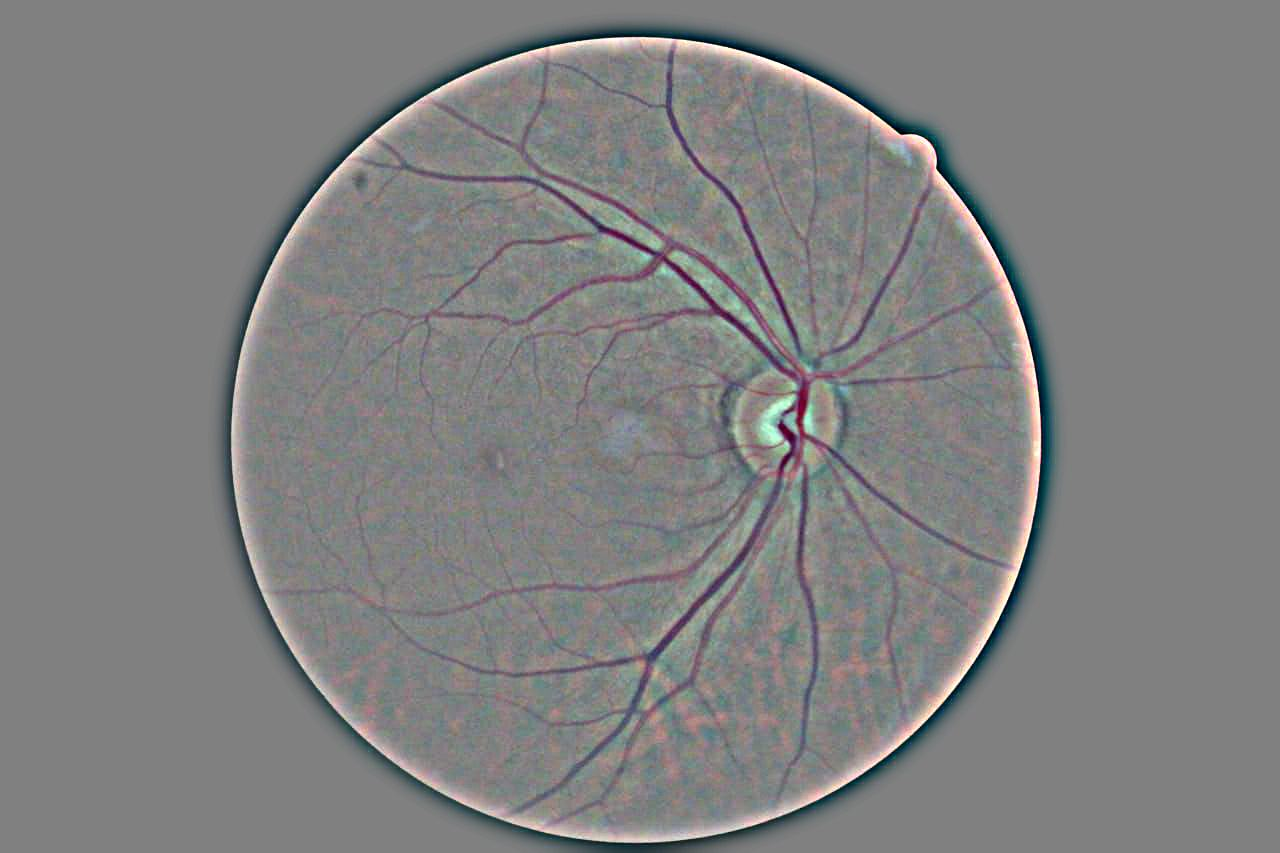
\includegraphics[width=\textwidth, height=\textwidth]{figures/chapter4/Preprocessing/weighted.jpg}
        \caption{Overlapped}
    \end{subfigure}
    \hfill
     \begin{subfigure}[b]{0.24\textwidth}
        \centering
        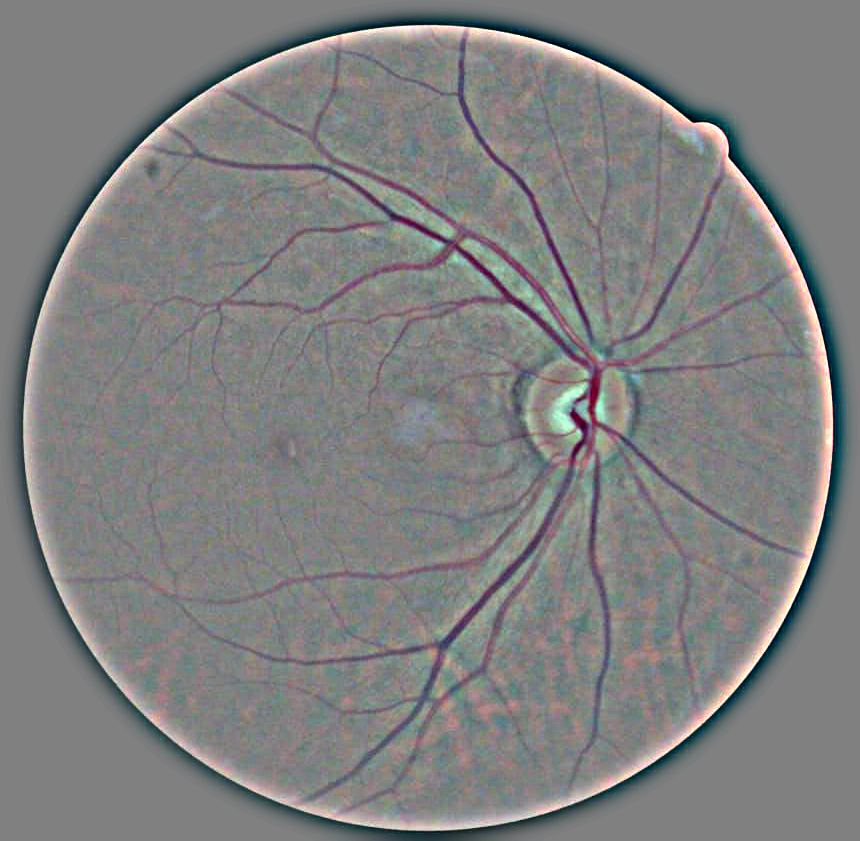
\includegraphics[width=\textwidth, height=\textwidth]{figures/chapter4/Preprocessing/cropped.jpg}
        \caption{Cropped}
    \end{subfigure}
    \caption{Process of preprocessing an image. The original image is rectangular, so it appears stretched when scaled to a squared image.}
    \label{fig:completePreprocess}
\end{figure}

The technique of adding Gaussian noise to images is a common technique in data augmentation, as it can make small details stand up and well-behaved noise can help the model become more robust. 

In its current shape, it behaves as a stochastic way to achieve local histogram normalization and in our proofs it has shown superior to other techniques, such as CLAHE \cite{pizer1987adaptive}. 

\Cref{fig:completePreprocess} shows the entire preprocessing process for an image, except for changes in scale. The application of Gaussian noise successfully highlights the blood vessels and the main anatomical structures, as the optic nerve. It also removes some undesirable effects, as the changes in brightness.

After the cropping process, the image can be scaled to a square without significant stretching, which is crucial since the model should be fed similarly sized images and as we said, the original images have remarkable different aspect ratios.

\Cref{fig:preprocess} shows the result of preprocessing several images. We note that the preprocessing brings out the lesions and the pathological stretch marked pattern and provide uniform results when applied to images with very different scales and light conditions.

While this method sacrifices most color information, we have found that color is dependent on the brightness conditions and does not contain diagnostic information by itself.

\begin{figure}[tb]
     \begin{subfigure}[b]{0.24\textwidth}
         \centering
         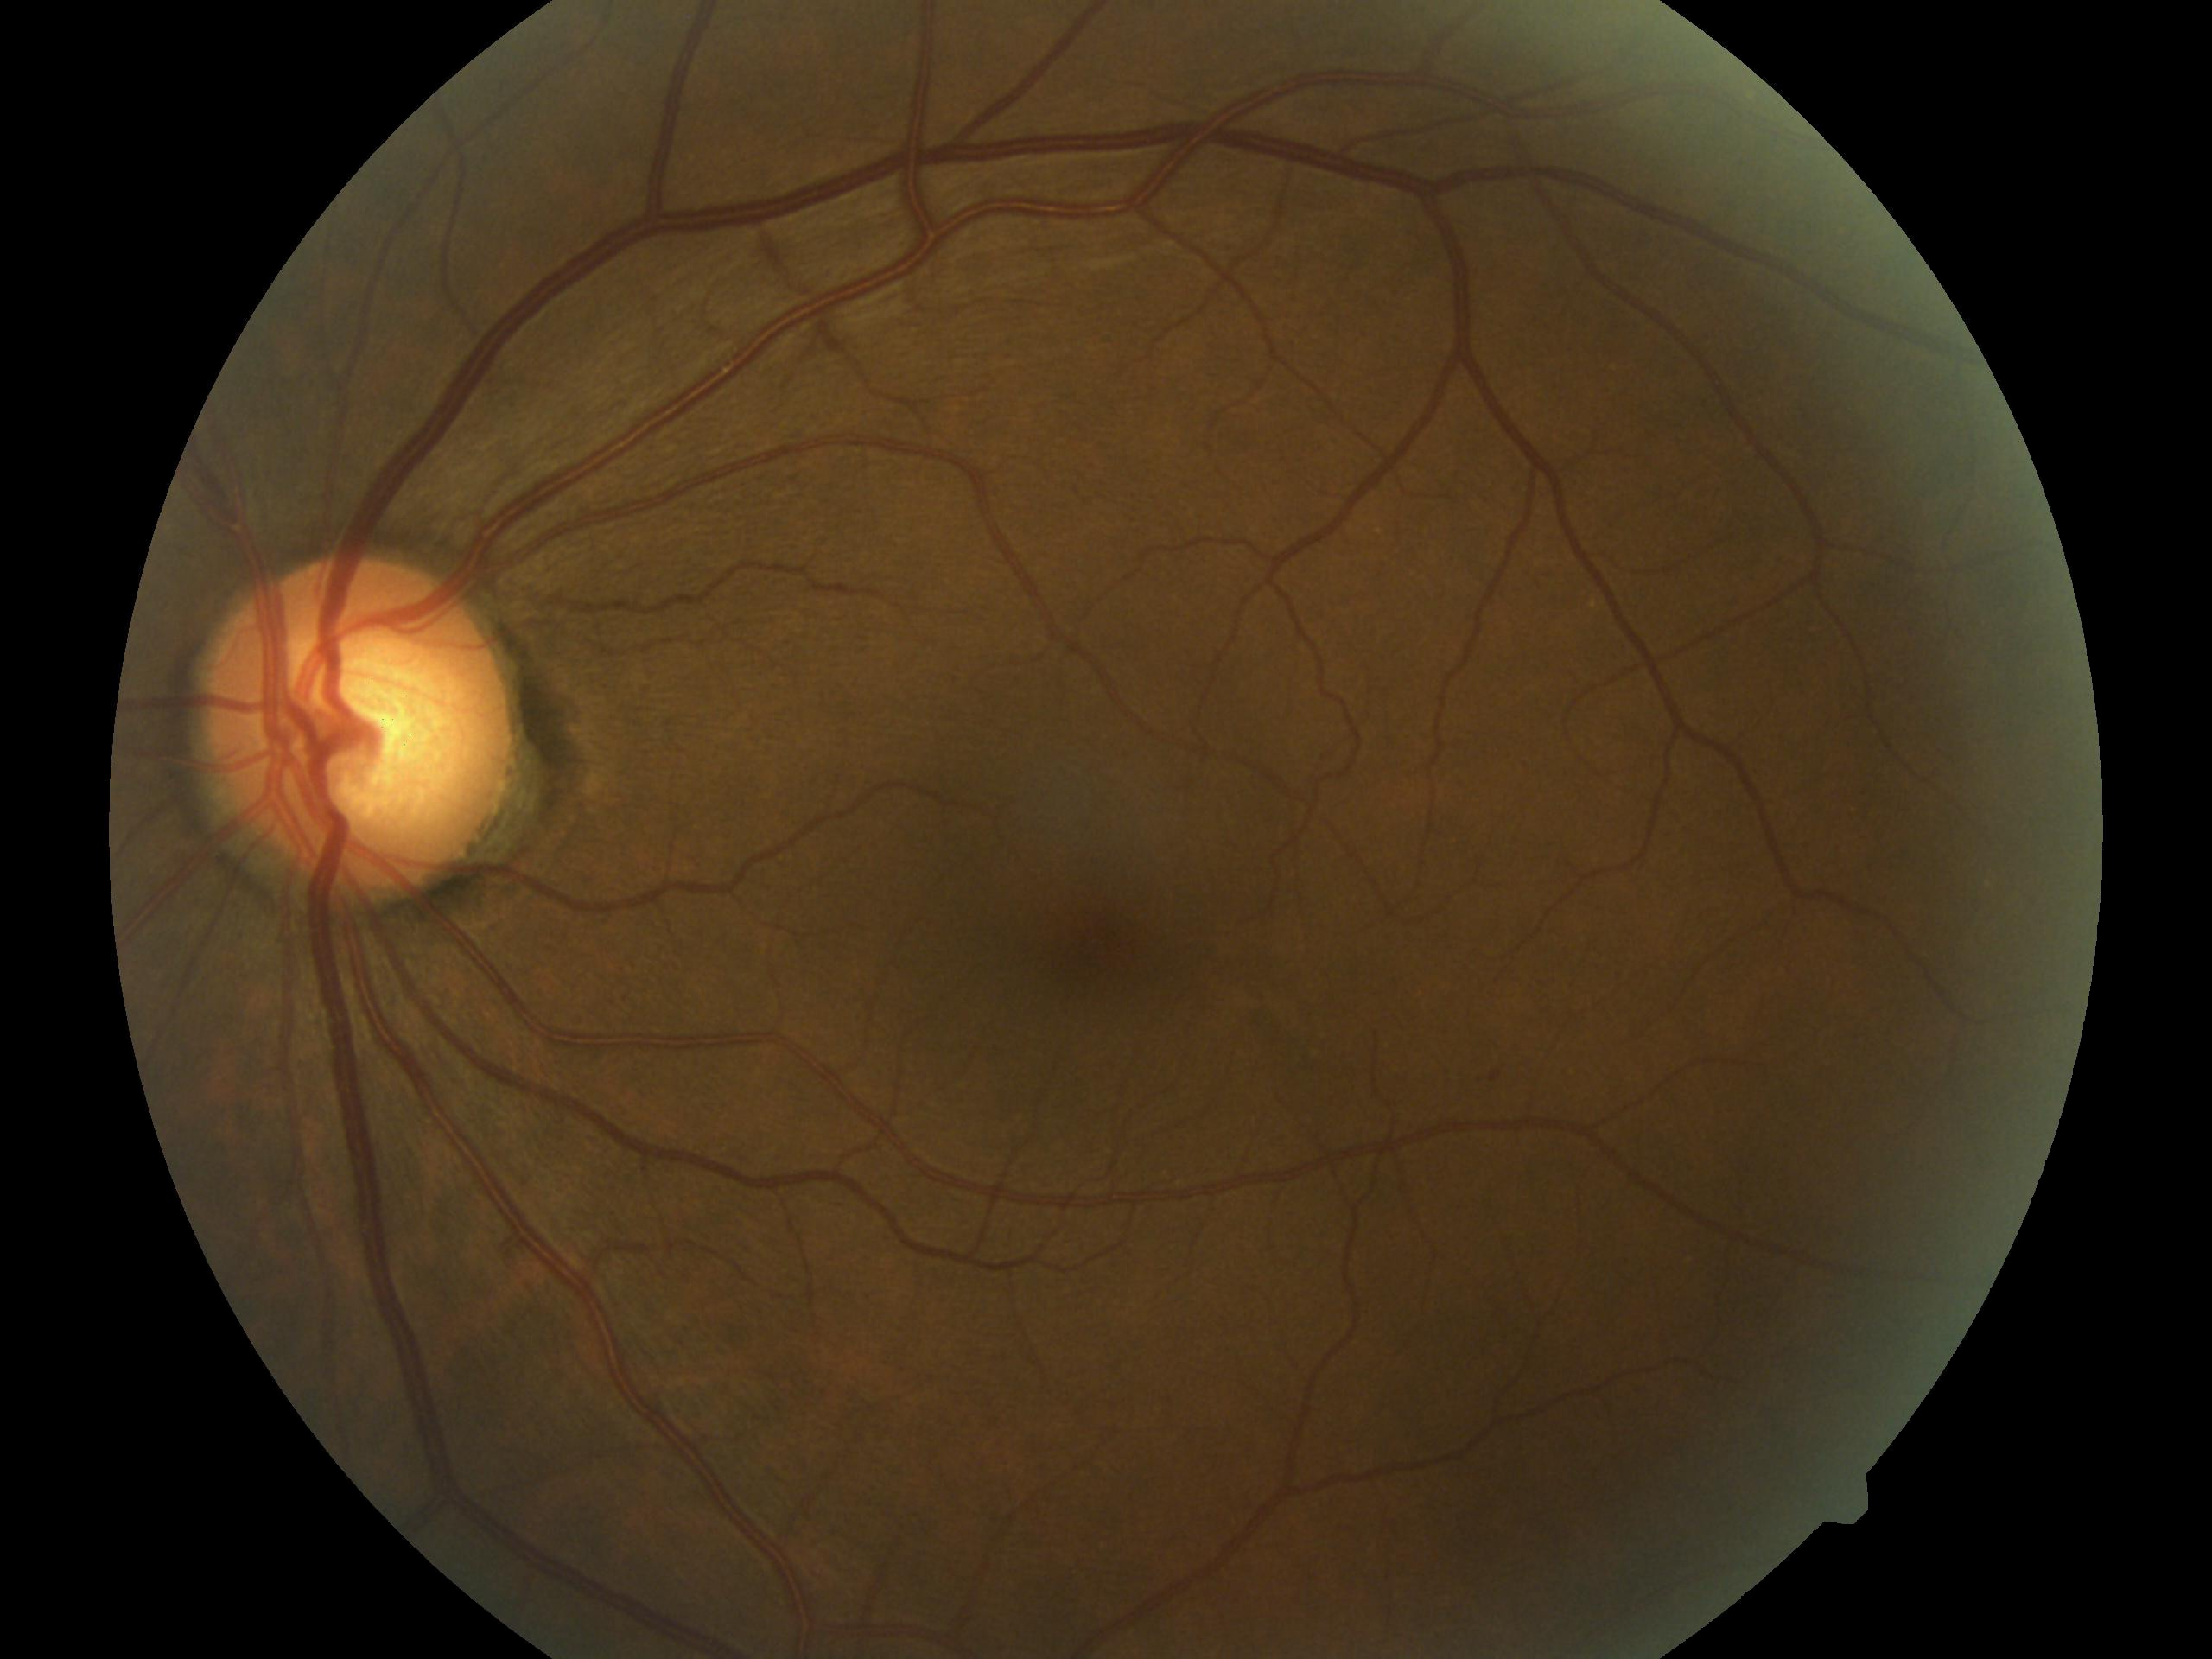
\includegraphics[width=\textwidth, height=\textwidth]{figures/chapter4/Preprocessing/Ori/36_left.jpeg}
    \end{subfigure}
    \hfill
    \begin{subfigure}[b]{0.24\textwidth}
         \centering
         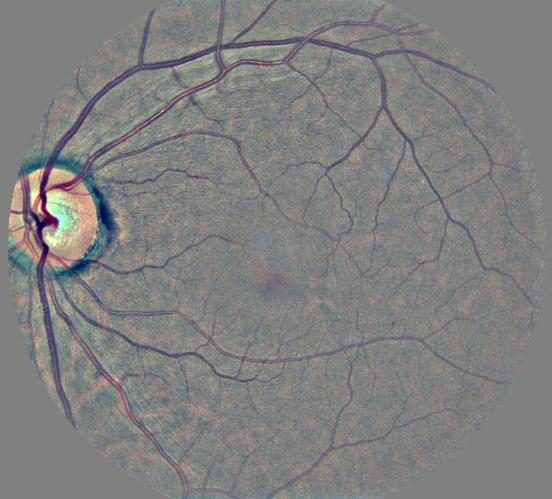
\includegraphics[width=\textwidth, height=\textwidth]{figures/chapter4/Preprocessing/Prep/36_left_prepr.jpeg}
    \end{subfigure}
    \hfill
    \begin{subfigure}[b]{0.24\textwidth}
         \centering
         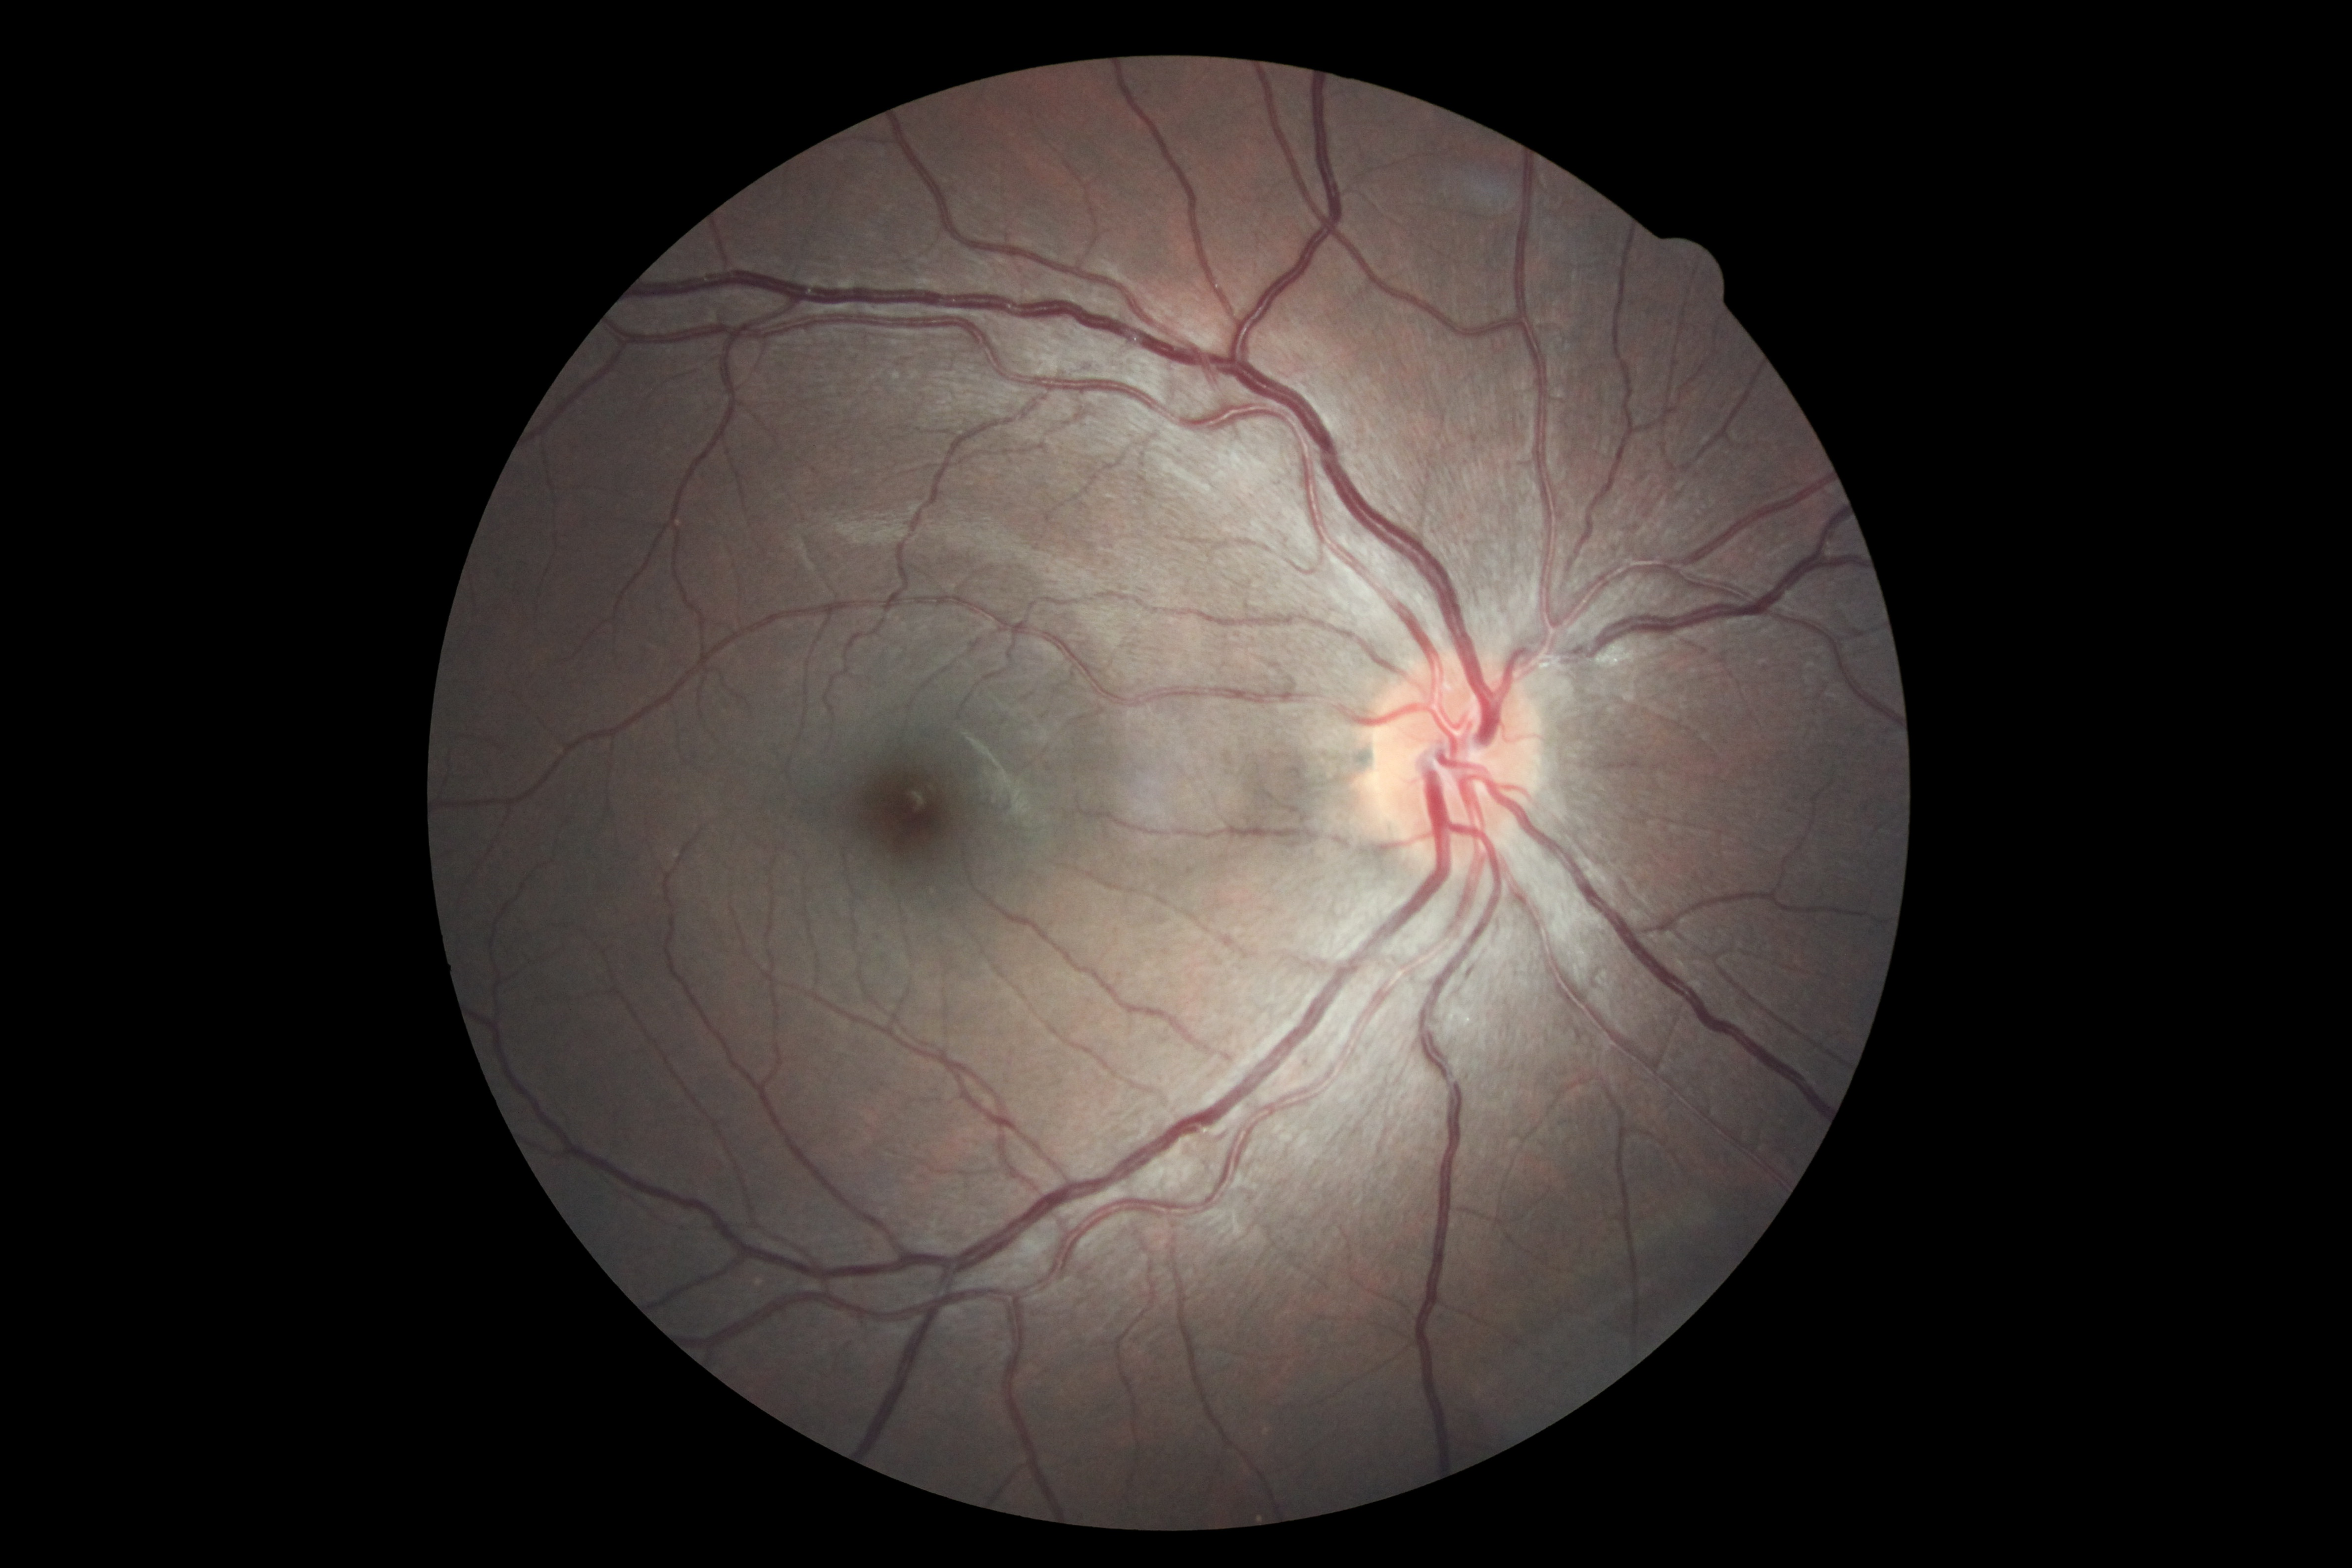
\includegraphics[width=\textwidth, height=\textwidth]{figures/chapter4/Preprocessing/Ori/114_right.jpeg}
    \end{subfigure}
    \hfill
    \begin{subfigure}[b]{0.24\textwidth}
         \centering
         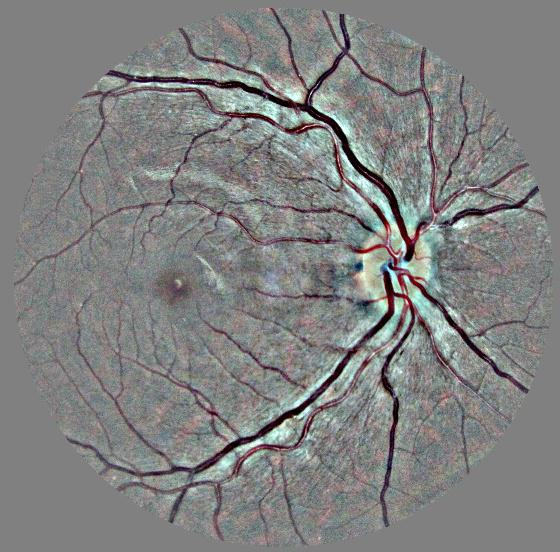
\includegraphics[width=\textwidth, height=\textwidth]{figures/chapter4/Preprocessing/Prep/114_right.jpeg}
     \end{subfigure}

    \bigskip
     \begin{subfigure}[b]{0.24\textwidth}
         \centering
         \includegraphics[width=\textwidth, height=\textwidth]{figures/chapter4/Preprocessing/Ori/41_left.jpeg}
    \end{subfigure}
    \hfill
    \begin{subfigure}[b]{0.24\textwidth}
        \centering
        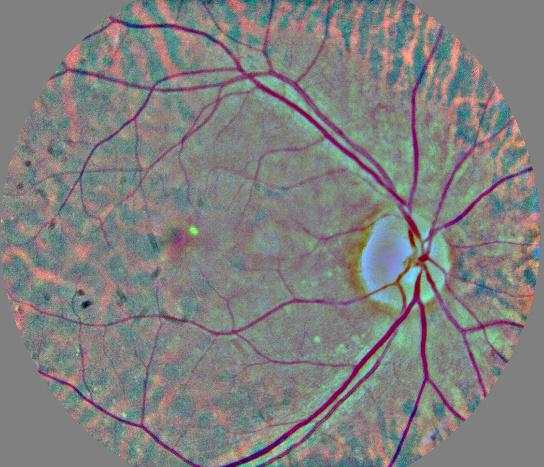
\includegraphics[width=\textwidth, height=\textwidth]{figures/chapter4/Preprocessing/Prep/41_left_crop.jpeg}
    \end{subfigure}
    \hfill
    \begin{subfigure}[b]{0.24\textwidth}
        \centering
        \includegraphics[width=\textwidth, height=\textwidth]{figures/chapter4/Preprocessing/Ori/294_left.jpeg}
    \end{subfigure}
    \hfill
    \begin{subfigure}[b]{0.24\textwidth}
        \centering
        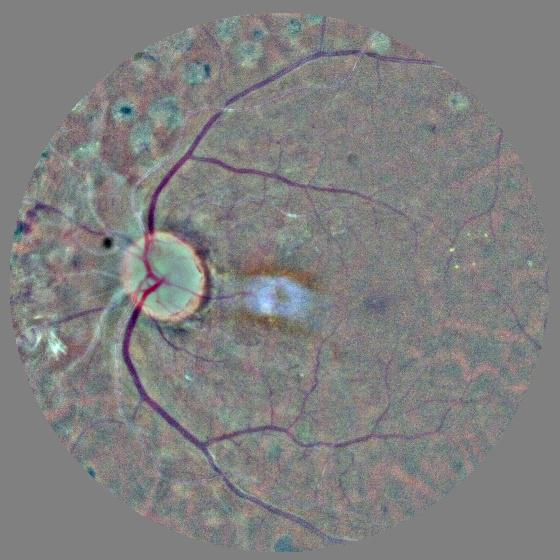
\includegraphics[width=\textwidth, height=\textwidth]{figures/chapter4/Preprocessing/Prep/294_left.jpeg}
     \end{subfigure}

    \bigskip
     \begin{subfigure}[b]{0.24\textwidth}
         \centering
         \includegraphics[width=\textwidth, height=\textwidth]{figures/chapter4/Preprocessing/Ori/54_right.jpeg}
         \caption{Original}
    \end{subfigure}
    \hfill
    \begin{subfigure}[b]{0.24\textwidth}
        \centering
        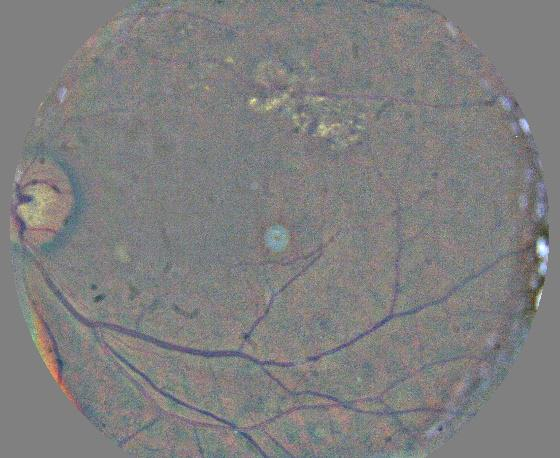
\includegraphics[width=\textwidth, height=\textwidth]{figures/chapter4/Preprocessing/Prep/54_right.jpeg}
        \caption{Processed}
    \end{subfigure}
    \hfill
    \begin{subfigure}[b]{0.24\textwidth}
        \centering
        \includegraphics[width=\textwidth, height=\textwidth]{figures/chapter4/Preprocessing/Ori/352_right.jpeg}
        \caption{Original}
    \end{subfigure}
    \hfill
    \begin{subfigure}[b]{0.24\textwidth}
        \centering
        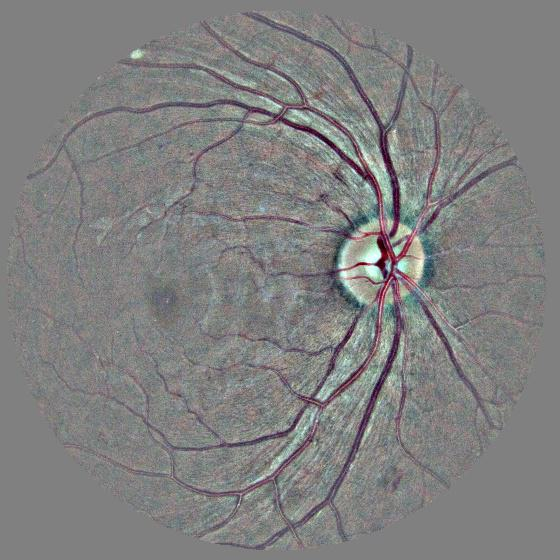
\includegraphics[width=\textwidth, height=\textwidth]{figures/chapter4/Preprocessing/Prep/352_right.jpeg}
        \caption{Processed}
     \end{subfigure}
    \caption{Result of preprocessing. It can be observed details like capillaries or lesions have
become more obvious and most of the illumination artifacts have disappeared.}
    \label{fig:preprocess}
\end{figure}

\section{Data augmentation}
Since we have limited data, it is convenient to use data augmentation techniques to create small variations of images. This will not only increase the effective size of the dataset, but also prevent overfitting and increase the robustness of the model.

By randomly applying transformations to an image before feeding them into the model, the model can become robust against rotations, reflections, or color variations of the images. We apply the following transformations (from the Albumentations open source library \cite{albumentations}) to each image with probability \( 0.5 \): scaling the image by a random factor in  \( (0.9, 1.1) \), rotating it by a random angle, flipping it vertically, horizontally or both. We do not include color or brightness transformation, as the preprocessing method removes the main of both from the original image. After this process, the image is scaled to the working resolution, that will usually depend on the concrete choice of the model.

To be able to process the images it is convenient that they are (approximately) normalized, so all components have a similar magnitude and the learning process is not affected by spurious differences of scales.

We apply normalization after data augmentation and immediately before feeding the image to the model. The normalized image \( I' \) is calculated from the augmented image \( I \) as:
\[I' = \frac{I - \mu}{\sigma}\]
where \( \mu \) is the mean and \( \sigma \) is the standard deviation, calculated separately for each channel over the whole training set. 